\documentclass[fleqn,11pt,letter]{article}
\setlength{\textwidth}{17.5cm}
\setlength{\textheight}{23.2cm}
\setlength{\hoffset}{-2.0cm}
\setlength{\voffset}{-2.5cm}

\usepackage{graphicx}
\usepackage{lastpage}
% \usepackage{datetime}
\usepackage{fancyheadings}
\usepackage{float}
\usepackage{caption}
\usepackage{subcaption}
\usepackage{color}
\usepackage[utf8]{inputenc}
\usepackage[T1]{fontenc}
\usepackage{textcomp}
\usepackage{gensymb}
\usepackage{amsmath}

\usepackage{multirow}
\usepackage{hyperref}


\pagestyle{fancy}

\def\today
{\number\day.\space \ifcase\month\or
January\or
February\or
March\or
April\or
May\or
June\or
July\or
August\or
September\or
October\or
November\or
December\fi,\space
\number\year}

%%%%
\newcount\hh
\newcount\mm
\mm=\time
\hh=\time
\divide\hh by 60
\divide\mm by 60
\multiply\mm by 60
\mm=-\mm
\advance\mm by \time
\def\hhmm{\number\hh:\ifnum\mm<10{}0\fi\number\mm}

%%%%%
\lhead{\small \it Verification for Real ESSI Simulator}
\chead{\small \it }
\rhead{\small \it \thepage{} of \pageref{LastPage} }
%
\lfoot{\small \it UC Davis}
\rfoot{\small \it \today, \hhmm}
\cfoot{\small \it Draft}
\addtolength{\headheight}{14pt}


\newcommand{\tabincell}[2]{\begin{tabular}{@{}#1@{}}#2\end{tabular}}





\begin{document}

%%%%%%%%%%%%%%%%%%%%Start Here%%%%%%%%%%%%%%%%%%%%%%%
%%%%%%%%%%%%%%%%%%%%Start Here%%%%%%%%%%%%%%%%%%%%%%%
%%%%%%%%%%%%%%%%%%%%Start Here%%%%%%%%%%%%%%%%%%%%%%%
%-------------------------------------------------------------------------------------------------------------%
%-------------------------------------------------------------------------------------------------------------%

\thispagestyle{fancy}


\tableofcontents{}









\newpage
% \begin{center}
%   \Large\textbf{Verification for 8NodeBrick}
% \end{center}
%\title{Scientific computing in geotechnical engineering}
%\maketitle

\section{Verification of 8NodeBrick elements}
\vskip 24pt

\subsection{Verification of 8NodeBrick cantilever beams}




Problem description: Length=6m, Width=1m, Height=1m, Force=100N, E=1E8Pa, $\nu=0.0$. The force direction was shown in Figure (\ref{fig Problem description for cantilever beams}). 

\begin{figure}[H]
  \centering
  \includegraphics[width=7cm]{../Figure_files/8NodeBrick/cantilever_6.pdf}
  \caption{Problem description for cantilever beams}
  \label{fig Problem description for cantilever beams}
\end{figure}


Theoretical displacement (bending and shear deformation):
\begin{equation}
  \begin{aligned}
  d &=\frac{FL^3}{3EI}+\frac{FL}{GA} \\ 
    &= \frac{100 N \times 6^3 m^3}{3\times 10^8 N/m^2 \times \frac{1}{12} m^4}+ 
    \frac{100 N\times 6 m}{5\times 10^7 N/m^2\times 1 m^2} \\ 
    &=8.64\times 10^{-4} m + 0.12 \times 10^{-4} m  \\
   & =8.76\times 10^{-4} \ m
   \end{aligned}
\end{equation}



Numerical model:



The 8NodeBrick elements were shown in Figure (\ref{fig 8NodeBrick elements for cantilever beams}).

\begin{figure}[H]
  \centering
  \begin{subfigure}{0.5\textwidth}
    \centering
    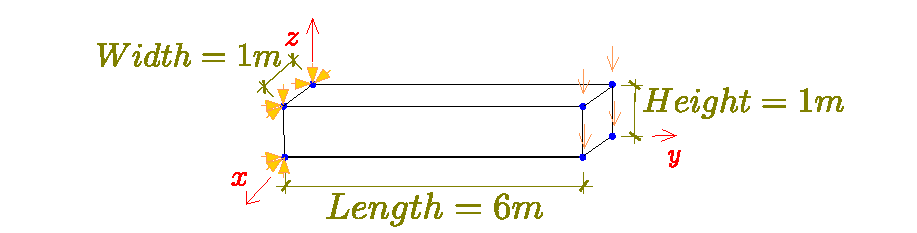
\includegraphics[width=9cm]{../Figure_files/8NodeBrick/beam_8brick_1div.pdf}
    \caption{One 8NodeBrick element}
  \end{subfigure}
  \vskip 8pt
  \begin{subfigure}{0.5\textwidth}
    \centering
    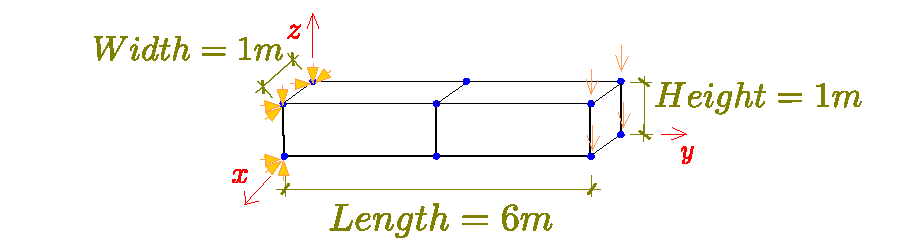
\includegraphics[width=9cm]{../Figure_files/8NodeBrick/beam_8brick_2div.pdf}
    \caption{Two 8NodeBrick elements}
  \end{subfigure}
  \vskip 8pt
  \begin{subfigure}{0.5\textwidth}
    \centering
    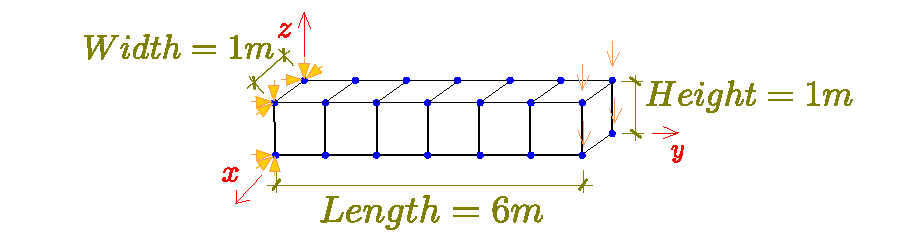
\includegraphics[width=9cm]{../Figure_files/8NodeBrick/beam_8brick_6div.pdf}
    \caption{Six 8NodeBrick elements}
  \end{subfigure}
  \captionsetup{justification=centering,margin=3cm}
  \caption{8NodeBrick elements for cantilever beams}
  \label{fig 8NodeBrick elements for cantilever beams}
\end{figure}


% \begin{figure}[H]
%   \centering
%   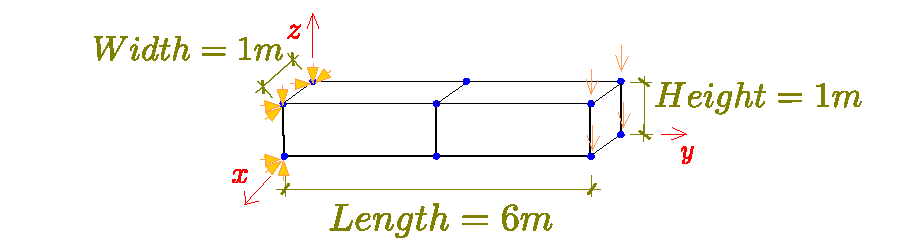
\includegraphics[width=9cm]{../Figure_files/8NodeBrick/beam_8brick_2div.pdf}
%   % \caption{}
%   % \label{}
% \end{figure}

% \begin{figure}[H]
%   \centering
%   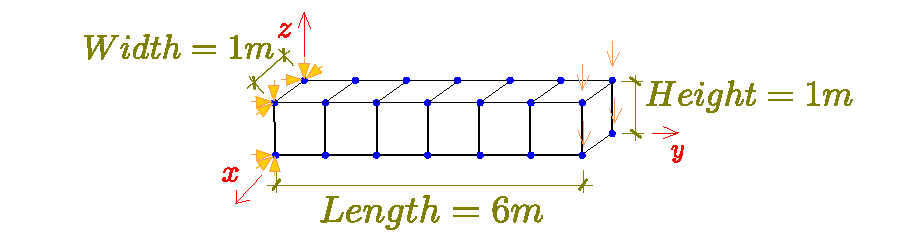
\includegraphics[width=9cm]{../Figure_files/8NodeBrick/beam_8brick_6div.pdf}
%   % \caption{}
%   % \label{}
% \end{figure}




All the ESSI results were listed in Table (\ref{table 8NodeBrick cantilever beams results for different element number}). 
The theoretical solution is 8.760E-04 $m$.
\begin{table}[H]
  \centering
    \caption{Results for 8NodeBrick cantilever beams of different element numbers}
    \begin{tabular}{|c|c|c|c|}
      \hline
      Element number & 1        & 2        & 6         \\  \hline
      8NodeBrick     & 4.61E-05 $m$ & 1.59E-04 $m$ & 5.84E-04 $m$     \\ \hline
      Error           & 94.74\%  & 81.82\%  & 33.33\%           \\ 
      \hline 
    \end{tabular}
    \label{table 8NodeBrick cantilever beams results for different element number}
\end{table}

The errors were plotted in Figure (\ref{fig error 8NodeBrick cantilever beam for different element number}).
\begin{figure}[H]
  % \centering
  % \begin{subfigure}{0.5\textwidth}
    \centering
    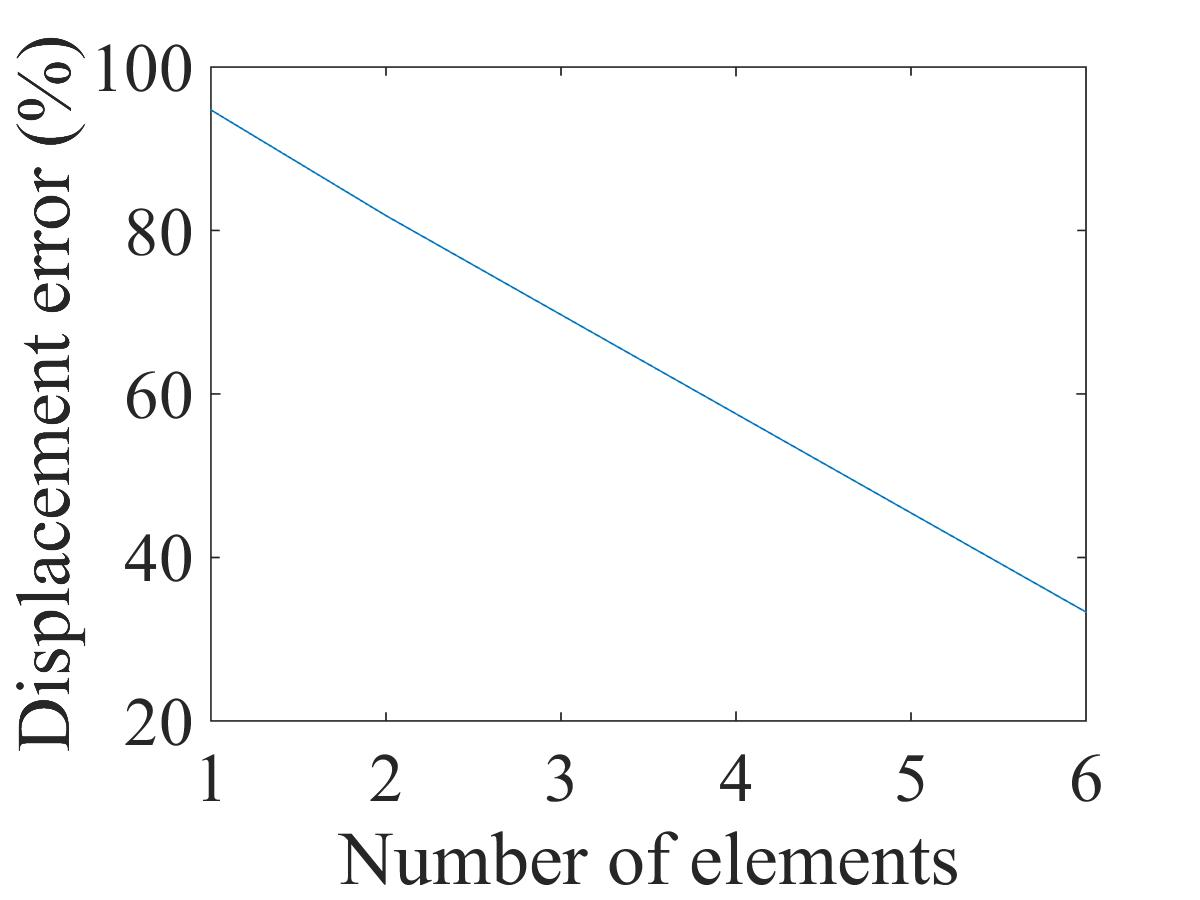
\includegraphics[width=6cm]{../Figure_files/8NodeBrick/error8brick_beam_different_element_number.jpeg}
  % \end{subfigure}
  % \begin{subfigure}{0.5\textwidth}
    % \centering
    % 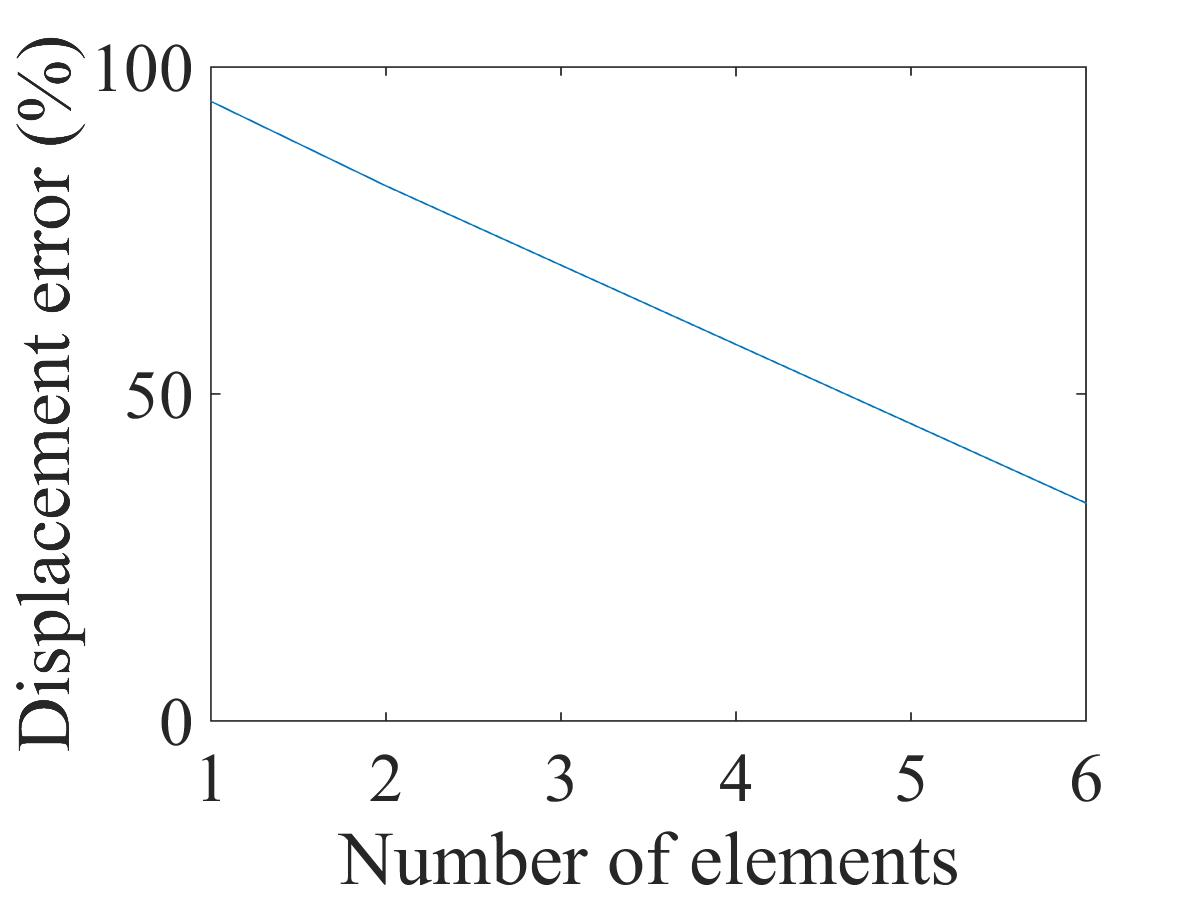
\includegraphics[width=7cm]{../Figure_files/8NodeBrick/error8brick_beam_different_element_number100.jpeg}
  % \end{subfigure}
  \captionsetup{justification=centering,margin=3cm}
  \caption{8NodeBrick cantilever beam for different element number\\
    Displacement error   versus   Number of elements}
  \label{fig error 8NodeBrick cantilever beam for different element number}
\end{figure}







The ESSI model fei files for the table above are \href{https://github.com/yuan-energy/ESSI_Verification/blob/master/8NodeBrick/cantilever_different_element_number/cantilever_different_element_number.tar.gz?raw=true}{here}






\newpage
\subsection{Verification of 8NodeBrick square plate with four edges clamped}

Problem description: Length=20m, Width=20m, Height=1m, Force=100N, E=1E8Pa, $\nu=0.3$. 

The four edges are clamped. 

The load is the uniform normal pressure on the whole plate. 


The plate flexural rigidity is 
\begin{equation}
  D=\frac{Eh^3}{12(1-\nu^2)}=\frac{10^8 N/m^2 \times 1^3 m^3 }{12 \times (1-0.3^2) }= 9.1575 \times 10^6 \ N\cdot m
\end{equation}
The theoretical solution is 
\begin{equation}
  d=\alpha_c \frac{q a^4}{D}=0.00406\times \frac{100 N/m^2 \times 20^4 m^4}{9.1575 \times 10^6 \ N\cdot m}=2.2015\times 10^{-3} m
\end{equation}

where $\alpha_c$ is a coefficient, which depends on the ratio of plate length to width. In this problem, the coefficient\footnote{Stephen Timoshenko, Theory of plates and shells (2nd edition). MrGRAW-Hill Inc, page120, 1959.} $\alpha_c$ is 0.00406.


The 8NodeBrick were shown in Figure (\ref{fig 8NodeBrick edges clamped square plate with element side length 10m }) - (\ref{fig 8NodeBrick edges clamped square plate with element side length 0.25m }). 


\begin{figure}[H]
  \centering
  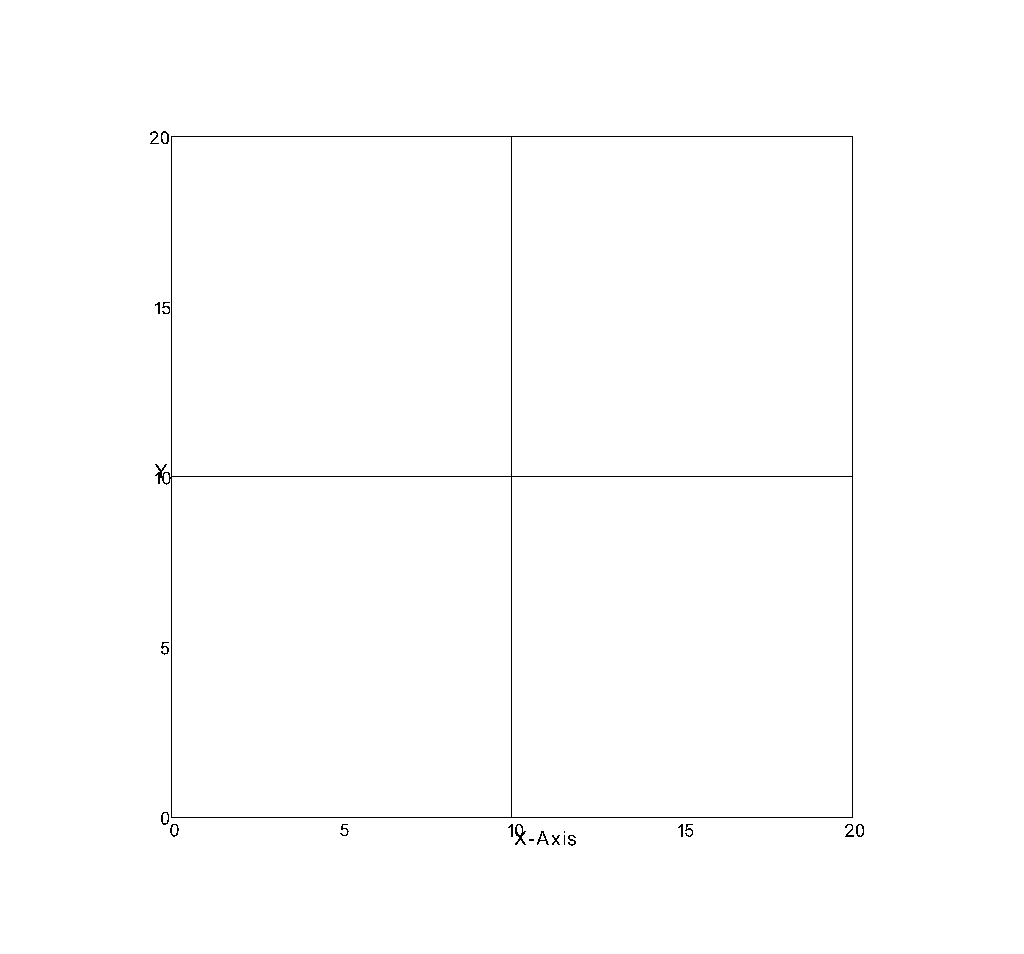
\includegraphics[width=11cm]{../Figure_files/8NodeBrick/square_plate1.png}
  \caption{8NodeBrick edge clamped square plate with element side length 10m }
  \label{fig 8NodeBrick edges clamped square plate with element side length 10m }
\end{figure}

\newpage

\begin{figure}[H]
  \centering
  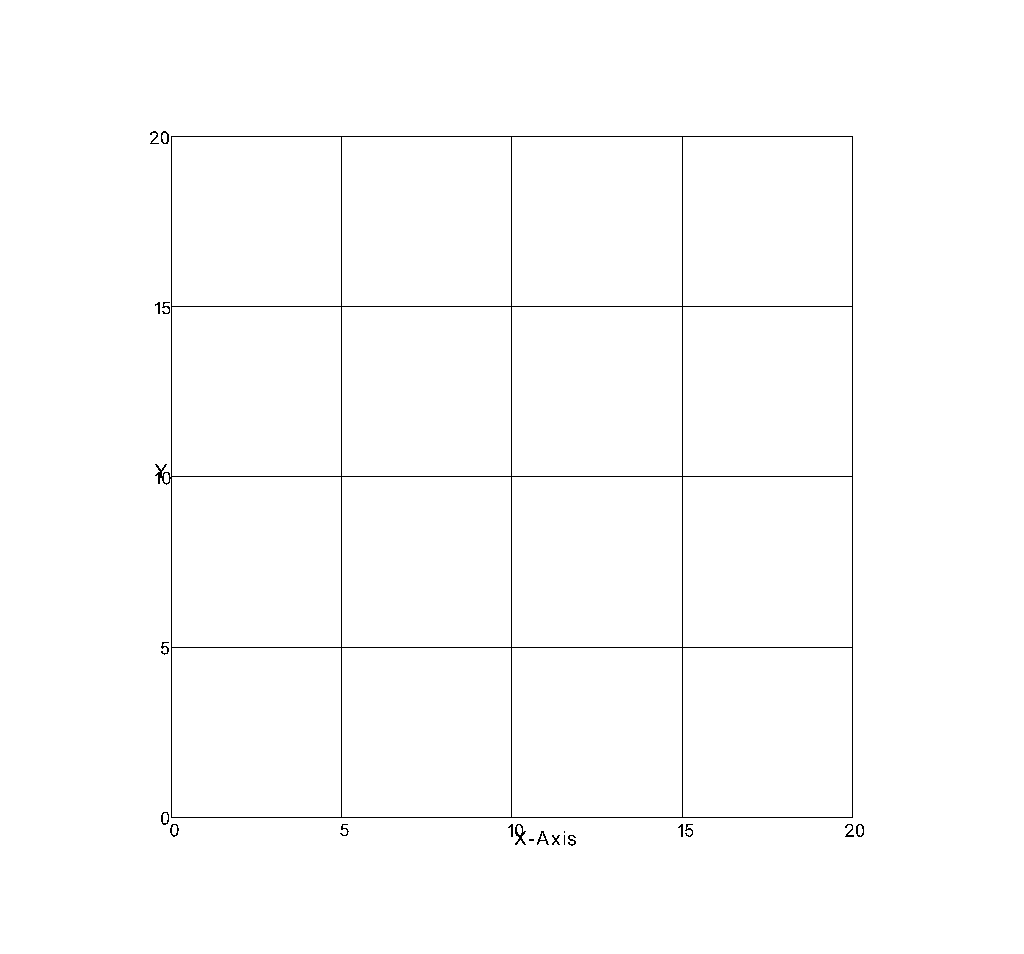
\includegraphics[width=11cm]{../Figure_files/8NodeBrick/square_plate2.png}
  \caption{8NodeBrick edge clamped square plate with element side length 5m }
  \label{fig 8NodeBrick edges clamped square plate with element side length 5m }
\end{figure}


\begin{figure}[H]
  \centering
  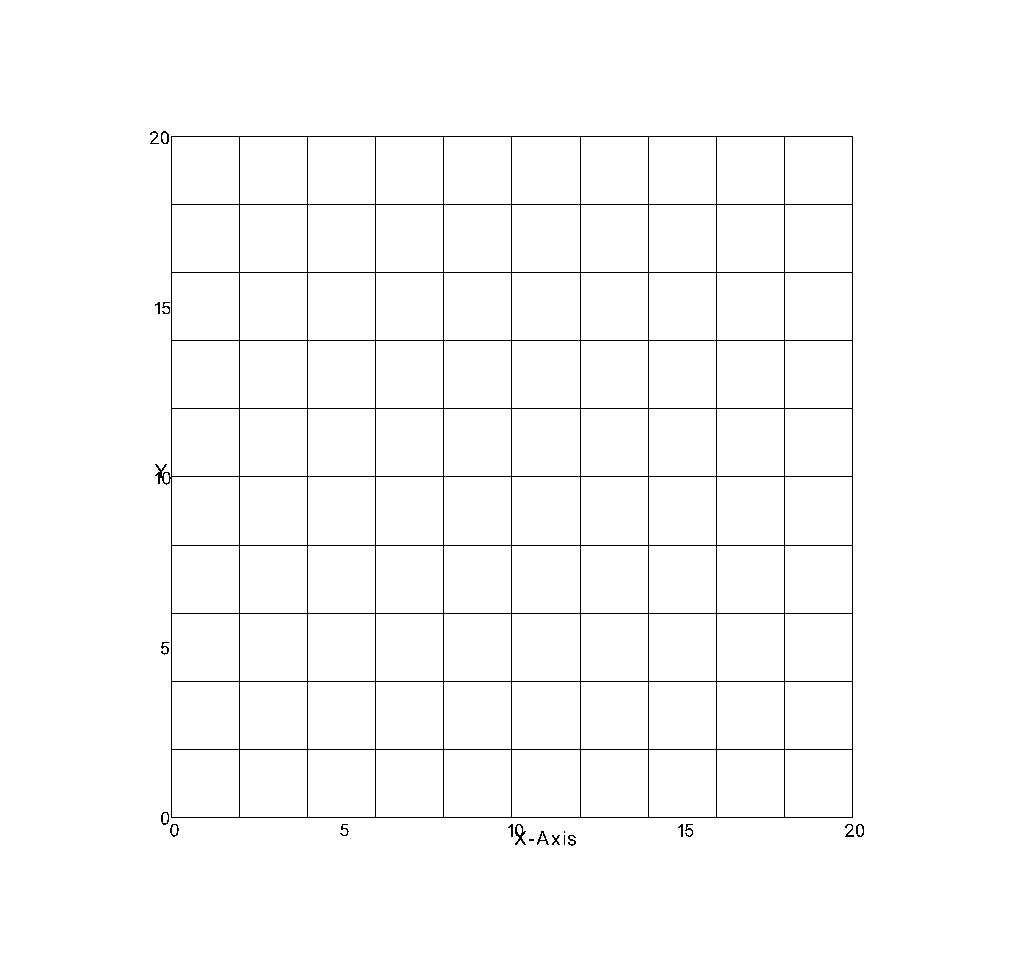
\includegraphics[width=11cm]{../Figure_files/8NodeBrick/square_plate3.png}
  \caption{8NodeBrick edge clamped square plate with element side length 2m }
  \label{fig 8NodeBrick edges clamped square plate with element side length 2m }
\end{figure}

\newpage

\begin{figure}[H]
  \centering
  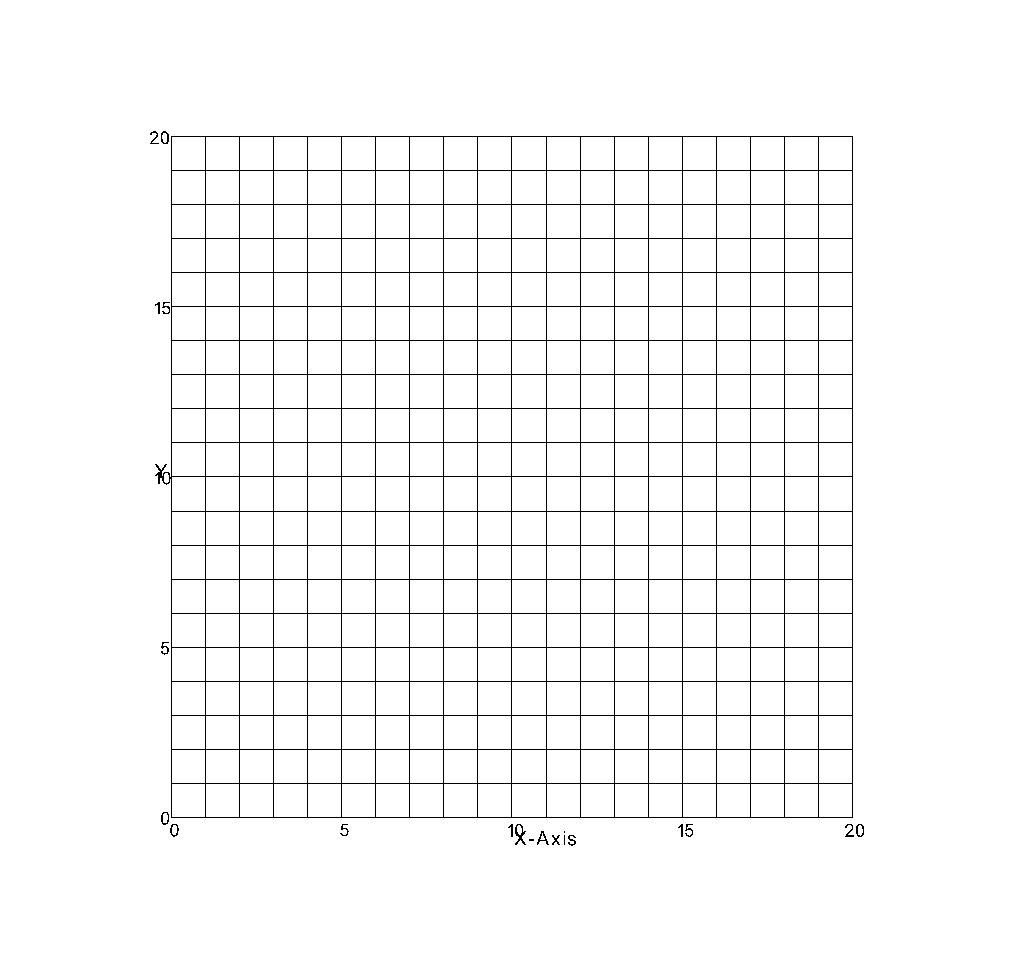
\includegraphics[width=11cm]{../Figure_files/8NodeBrick/square_plate4.png}
  \caption{8NodeBrick edge clamped square plate with element side length 1m }
  \label{fig 8NodeBrick edges clamped square plate with element side length 1m }
\end{figure}


\begin{figure}[H]
  \centering
  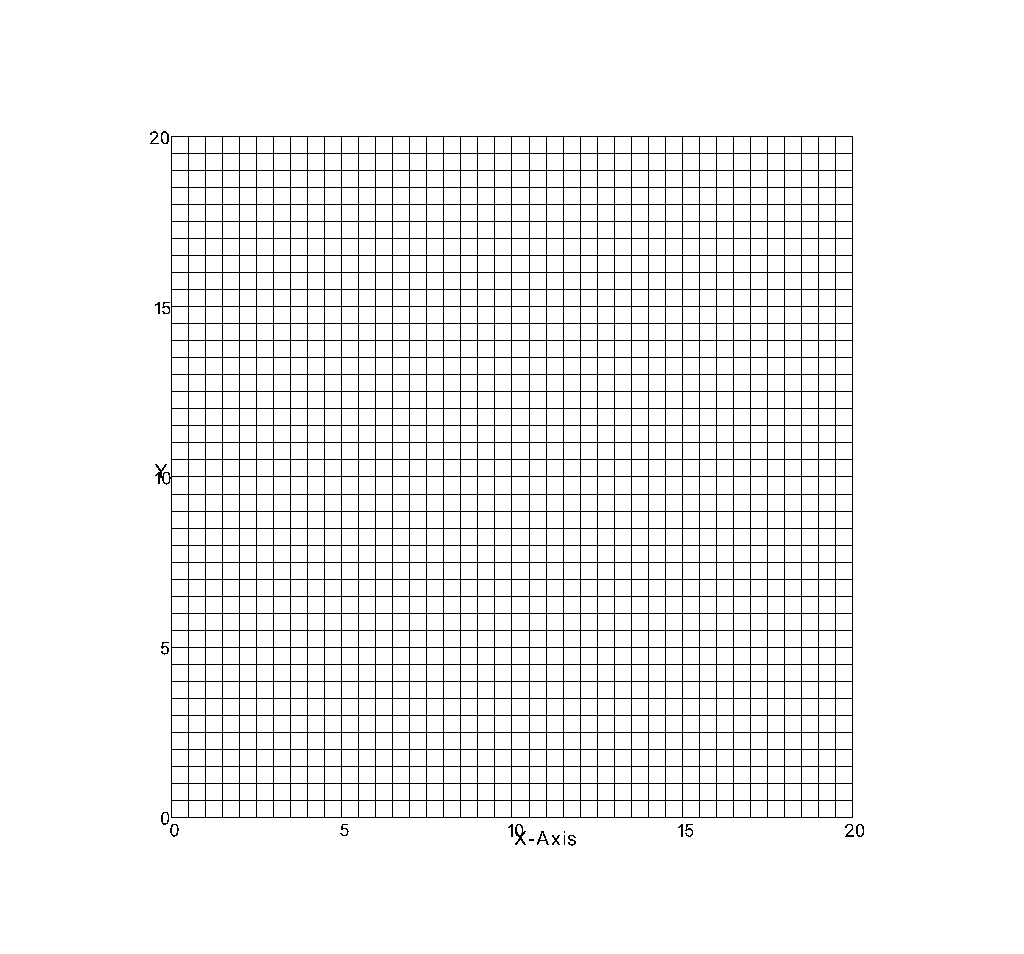
\includegraphics[width=11cm]{../Figure_files/8NodeBrick/square_plate5.png}
  \caption{8NodeBrick edge clamped square plate with element side length 0.5m }
  \label{fig 8NodeBrick edges clamped square plate with element side length 0.5m }
\end{figure}

\newpage

\begin{figure}[H]
  \centering
  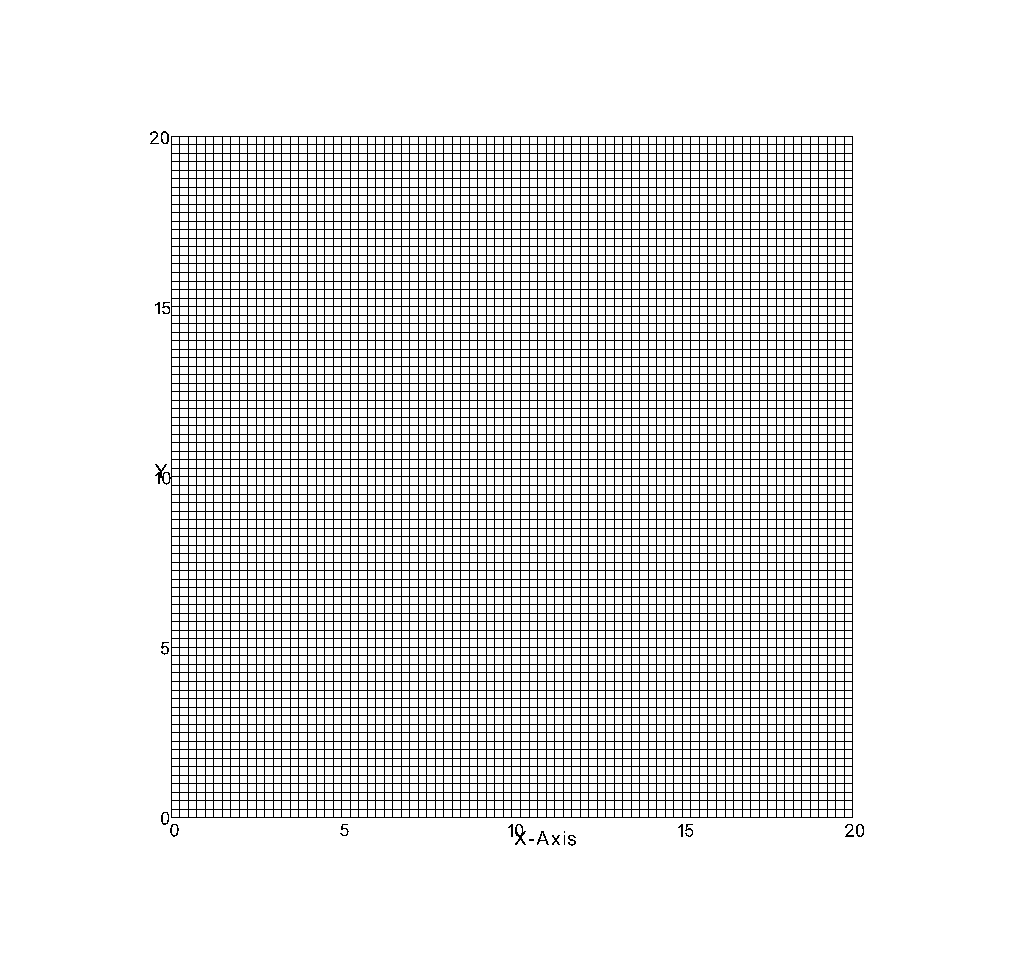
\includegraphics[width=11cm]{../Figure_files/8NodeBrick/square_plate6.png}
  \caption{8NodeBrick edge clamped square plate with element side length 0.25m }
  \label{fig 8NodeBrick edges clamped square plate with element side length 0.25m }
\end{figure}



The results were listed in Table (\ref{table Results for 8NodeBrick square plate with four edges clamped}).

\begin{table}[H]
  \centering
  \caption{Results for 8NodeBrick square plate with four edges clamped}
  \label{table Results for 8NodeBrick square plate with four edges clamped}
\begin{tabular}{|c|c|c|c|c|}
\hline
Element type     & 8NodeBrick     & 8NodeBrick     & 8NodeBrick     &  \multirow{3}{*}{\tabincell{c}{Theoretical \\ displacement}} \\ \cline{1-4}
Number of layers & 1layer         & 2layers         & 4layers         &          \\ \cline{1-4}
Element side length & Height:1.00$m$ & Height:0.50$m$ & Height:0.25$m$ &          \\ \hline
10$m$            & 9.75E-05  $m$  & 9.75E-05  $m$  & 9.75E-05 $m$  & 2.20E-03 $m$ \\ \hline
5$m$             & 3.28E-04  $m$  & 3.32E-04  $m$  & 3.32E-04 $m$  & 2.20E-03 $m$ \\ \hline
2$m$             & 1.04E-03  $m$  & 1.10E-03  $m$  & 1.12E-03 $m$  & 2.20E-03 $m$ \\ \hline
1$m$             & 1.56E-03  $m$  & 1.74E-03  $m$  & 1.79E-03 $m$  & 2.20E-03 $m$ \\ \hline
0.5$m$           & 1.80E-03  $m$  & 2.30E-03  $m$  & 2.12E-03 $m$  & 2.20E-03 $m$ \\ \hline
0.25$m$          & 1.87E-03  $m$  & 2.14E-03  $m$  & 2.23E-03 $m$  & 2.20E-03 $m$ \\
\hline
\end{tabular}
\end{table}


The errors were listed in Table (\ref{table Errors for 8NodeBrick square plate with four edges clamped}).

\begin{table}[H]
  \centering
  \caption{Errors for 8NodeBrick square plate with four edges clamped}
  \label{table Errors for 8NodeBrick square plate with four edges clamped}
\begin{tabular}{|c|c|c|c|c|}
\hline
Element type     & 8NodeBrick     & 8NodeBrick     & 8NodeBrick      \\ \hline
Number of layers & 1layer         & 2layers         & 4layers          \\ \hline
Element side length & Height:1.00$m$ & Height:0.50$m$ & Height:0.25$m$  \\ \hline
10$m$            & 95.57\%        & 95.57\%        & 95.57\%        \\ \hline
5$m$             & 85.09\%        & 84.94\%        & 84.91\%        \\ \hline
2$m$             & 52.98\%        & 50.09\%        & 49.25\%        \\ \hline
1$m$             & 28.93\%        & 21.17\%        & 18.72\%        \\ \hline
0.5$m$           & 18.26\%        & 4.58\%         & 3.56\%         \\ \hline
0.25$m$          & 15.05\%        & 2.70\%         & 1.37\%         \\
\hline
\end{tabular}
\end{table}



% \begin{figure}[H]
%   % \centering
%   \begin{subfigure}{0.5\textwidth}
%     \centering
%     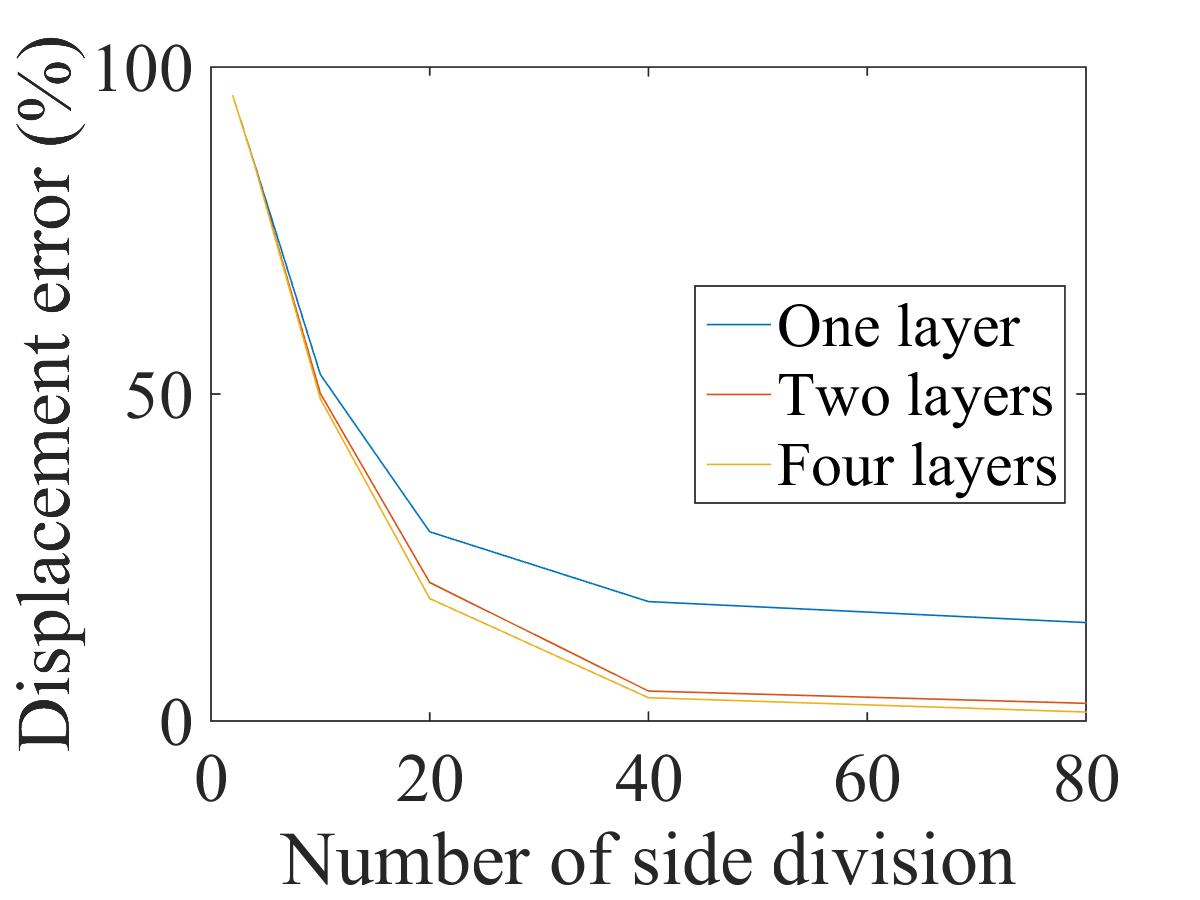
\includegraphics[width=6cm]{../Figure_files/8NodeBrick/error8brick_square_plate_clamped.jpeg}
%     \caption{Error scale 0\% - 80\%}
%   \end{subfigure}
%   \begin{subfigure}{0.5\textwidth}
%     \centering
%     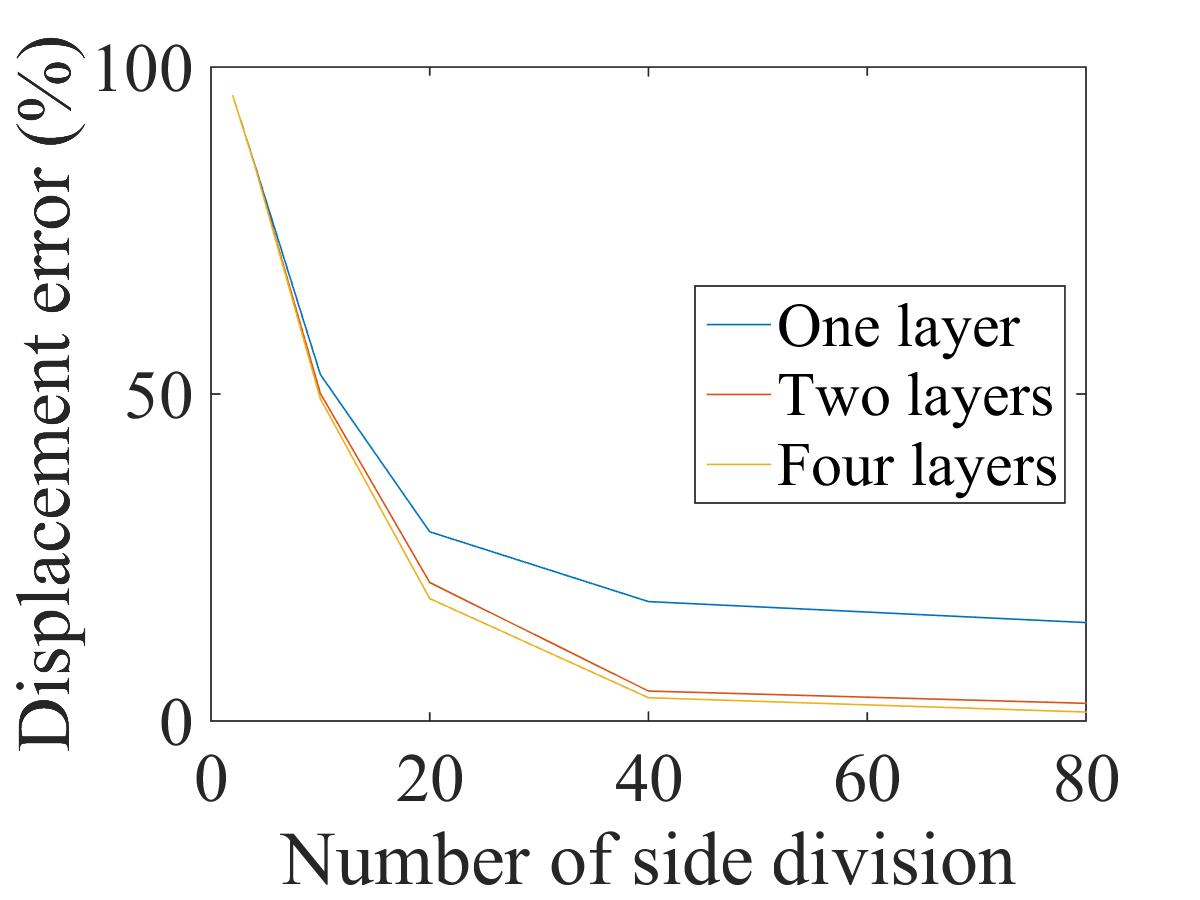
\includegraphics[width=6cm]{../Figure_files/8NodeBrick/error8brick_square_plate_clamped100.jpeg}
%     \caption{Error scale 0\% - 100\%}
%   \end{subfigure}
%   \captionsetup{justification=centering,margin=3cm}
%   \caption{Two sub}
%   % \caption{}
%   % \label{}
% \end{figure}


The errors were plotted in Figure (\ref{fig 8NodeBrick square plate with edge clamped}).
\begin{figure}[H]
  % \centering
    \centering
    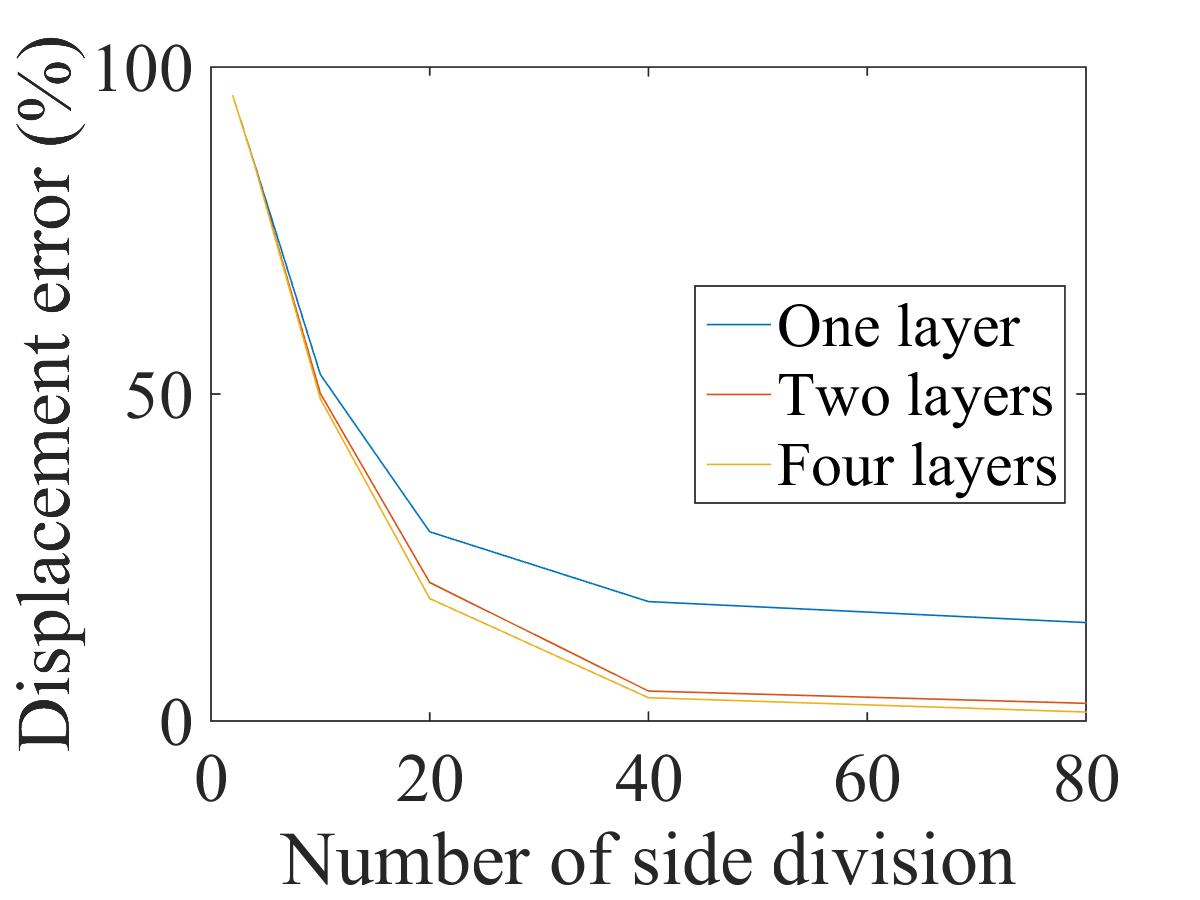
\includegraphics[width=6cm]{../Figure_files/8NodeBrick/error8brick_square_plate_clamped.jpeg}
  \captionsetup{justification=centering,margin=3cm}
  \caption{8NodeBrick square plate with edge clamped\\
      Displacement error   versus   Number of side division}
  \label{fig 8NodeBrick square plate with edge clamped}
\end{figure}



The ESSI model fei files for the table above are \href{https://github.com/yuan-energy/ESSI_Verification/blob/master/8NodeBrick/square_plate_clamped/square_plate_clamped.tar.gz?raw=true}{here}






% \newpage
% \begin{itemize}
%   \item \textbf{\emph{Square plate with edges clamped: different geometry}}
% \end{itemize}

% In the figures above, only the model with geometry $20m\times 20m \times 1m$ was drawed. In the ESSI models, the geometry $6m\times 6m \times 1m$ and the geometry $10m\times 10m \times 1m$ were also calculated. In three different geometry models, all the element sizes were $1m\times 1m \times 1m$.


% The ESSI displacement results were listed below.

% \begin{table}[H]
%   \centering
%   \begin{tabular}{|c|c|c|c|c|c|}
%     \hline 
%     \multirow{2}{*}{Element Type}  & \multirow{2}{*}{Number of layers}   
%        &  \multicolumn{3}{|c|}{Model geometry} \\       \cline{3-5}
%        & & 1:6 & 1:10 & 1:20 \\                              \hline
% 8NodeBrick &  2layers   &2.13E-04 $m$ & 1.54E-03 $m$ & 2.41E-02 $m$  \\ \hline
% 8NodeBrick &  4layers   &2.37E-04 $m$ & 1.71E-03 $m$ & 2.66E-02 $m$  \\ \hline
% \multicolumn{2}{|c|}{Theoretical}    &1.78E-05 $m$ & 1.38E-04 $m$ & 2.20E-03 $m$      \\ \hline
%   \end{tabular}
%   % \caption{}
% \end{table}



% The errors were listed below.

% \begin{table}[H]
%   \centering
%   \begin{tabular}{|c|c|c|c|c|c|}
%     \hline 
%     \multirow{2}{*}{Element Type}  & \multirow{2}{*}{Number of layers}   
%        &  \multicolumn{3}{|c|}{Model geometry} \\       \cline{3-5}
%        & & 1:6 & 1:10 & 1:20 \\                              \hline
% 8NodeBrick &  2layers   &3.58\% & 9.47\% & 11.77\%  \\ \hline
% 8NodeBrick &  4layers   &7.27\% & 0.19\% & 2.66\%   \\ \hline
%   \end{tabular}
%   % \caption{}
% \end{table}



































































\newpage
% \begin{center}
%   \Large\textbf{Verification for 27NodeBrick}
% \end{center}
%\title{Scientific computing in geotechnical engineering}
%\maketitle

\section{Verification of 27NodeBrick elements}
\subsection{Verification of 27NodeBrick cantilever beams}

% The model is \href{https://github.com/yuan-energy/test/archive/master.zip}{here}.

% The model is \href{https://github.com/yuan-energy/test/tree/master/example}{here}.

% The model is \href{https://github.com/yuan-energy/test/blob/master/example_2/example3.zip?raw=true}{here}.



Problem description: Length=6m, Width=1m, Height=1m, Force=100N, E=1E8Pa, $\nu=0.0$. The force direction was shown in Figure (\ref{fig Problem description for cantilever 27}). 

\begin{figure}[H]
  \centering
  \includegraphics[width=7cm]{../Figure_files/27NodeBrick/cantilever_6.pdf}
  \caption{Problem description for cantilever beams}
  \label{fig Problem description for cantilever 27}
\end{figure}


Theoretical displacement (bending and shear deformation):
\begin{equation}
  \begin{aligned}
  d &=\frac{FL^3}{3EI}+\frac{FL}{GA} \\ 
    &= \frac{100 N \times 6^3 m^3}{3\times 10^8 N/m^2 \times \frac{1}{12} m^4}+ 
    \frac{100 N\times 6 m}{5\times 10^7 N/m^2\times 1 m^2} \\ 
    &=8.64\times 10^{-4} m + 0.12 \times 10^{-4} m  \\
   & =8.76\times 10^{-4} \ m
   \end{aligned}
\end{equation}



Numerical model:

The 27NodeBrick elements were shown in Figure (\ref{fig 27NodeBrick elements for cantilever beams}).

\begin{figure}[H]
  \centering
  \begin{subfigure}{0.5\textwidth}
    \centering
    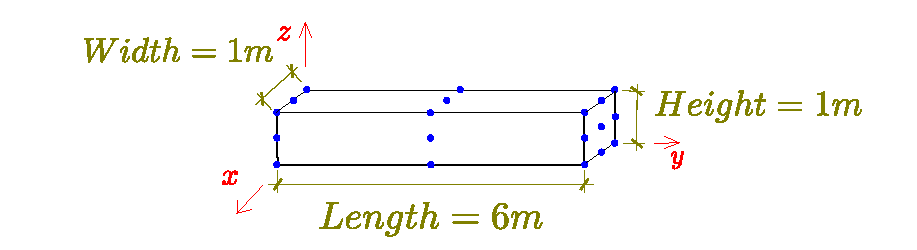
\includegraphics[width=9cm]{../Figure_files/27NodeBrick/beam_27brick_1div.pdf}
    \caption{One 27NodeBrick element}
  \end{subfigure}
  \vskip 8pt
  \begin{subfigure}{0.5\textwidth}
    \centering
    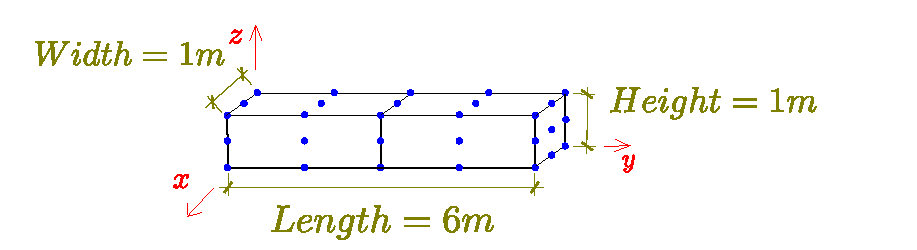
\includegraphics[width=9cm]{../Figure_files/27NodeBrick/beam_27brick_2div.pdf}
    \caption{Two 27NodeBrick elements}
  \end{subfigure}
  \vskip 8pt
  \begin{subfigure}{0.5\textwidth}
    \centering
    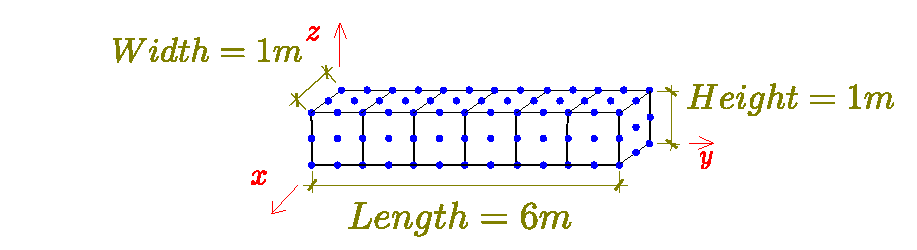
\includegraphics[width=9cm]{../Figure_files/27NodeBrick/beam_27brick_6div.pdf}
    \caption{Six 27NodeBrick elements}
  \end{subfigure}
  \captionsetup{justification=centering,margin=3cm}
  \caption{27NodeBrick elements for cantilever beams}
  \label{fig 27NodeBrick elements for cantilever beams}
\end{figure}



% 27NodeBrick element:
% \begin{figure}[H]
%   \centering
%   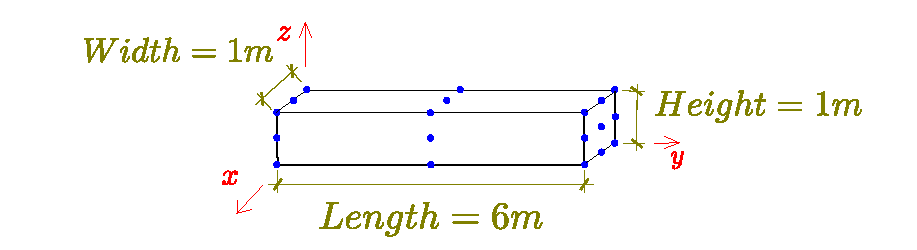
\includegraphics[width=9cm]{../Figure_files/27NodeBrick/beam_27brick_1div.pdf}
%   % \caption{}
%   % \label{}
% \end{figure}


% \begin{figure}[H]
%   \centering
%   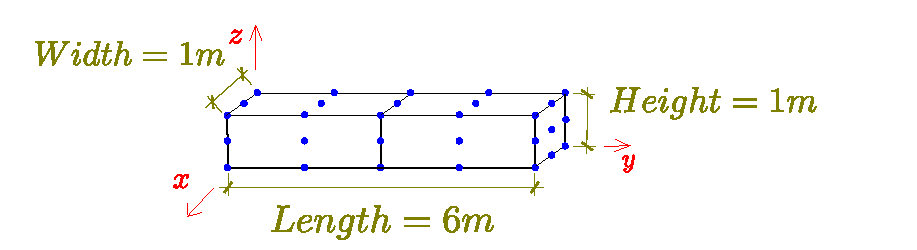
\includegraphics[width=9cm]{../Figure_files/27NodeBrick/beam_27brick_2div.pdf}
%   % \caption{}
%   % \label{}
% \end{figure}

% \begin{figure}[H]
%   \centering
%   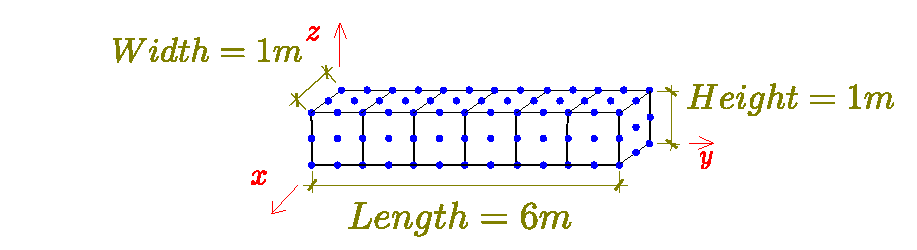
\includegraphics[width=9cm]{../Figure_files/27NodeBrick/beam_27brick_6div.pdf}
%   % \caption{}
%   % \label{}
% \end{figure}




All the ESSI results were listed in Table (\ref{table 27NodeBrick cantilever beams results for different element number}). 
\begin{table}[H]
  \centering
      \caption{Results for 27NodeBrick cantilever beams of different element numbers}
    \label{table 27NodeBrick cantilever beams results for different element number}
    \begin{tabular}{|c|c|c|c|}
      \hline
      Element number & 1        & 2        & 6         \\  \hline
      27NodeBrick     & 7.07E-04 $m$ & 8.50E-04 $m$ & 8.75E-04 $m$     \\ \hline
      Error           & 19.30\%  & 2.92\%   & 0.06\%    \\ 
      \hline 
    \end{tabular}
\end{table}



% \begin{figure}[H]
%   \centering
%   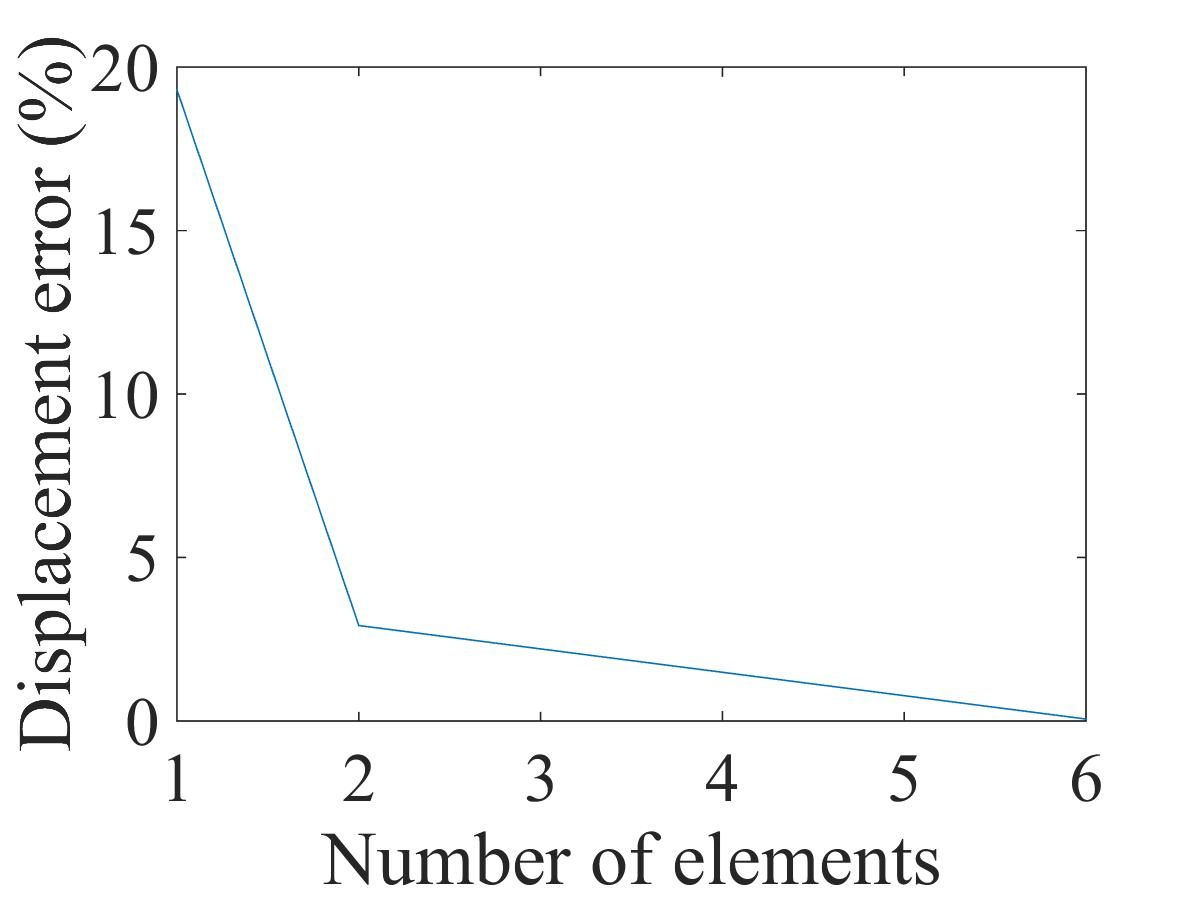
\includegraphics[width=9cm]{../Figure_files/27NodeBrick/error27brick_beam_different_element_number.jpeg}
%   % \caption{}
%   % \label{}
% \end{figure}
The errors were plotted in Figure (\ref{fig error 27NodeBrick cantilever beam for different element number}).

\begin{figure}[H]
  % \centering
  \begin{subfigure}{0.5\textwidth}
    \centering
    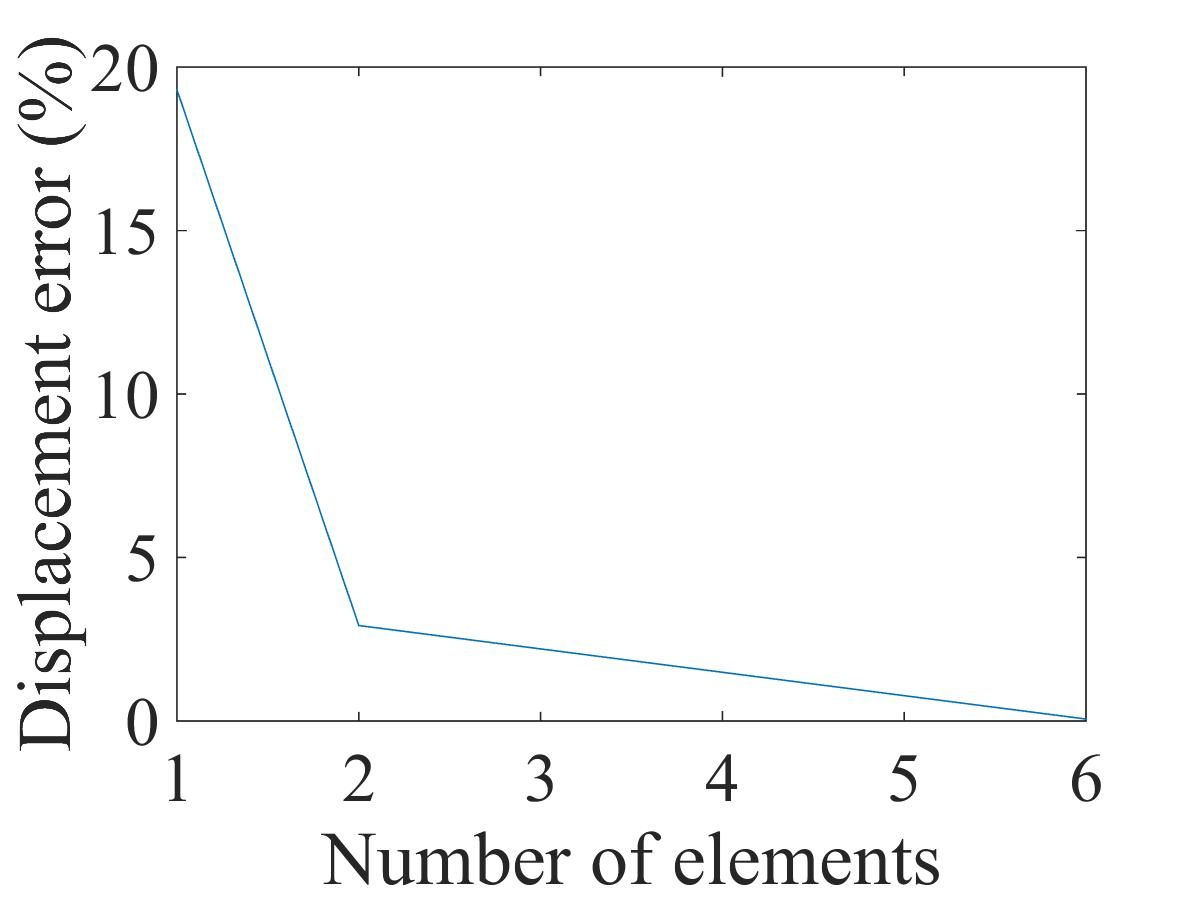
\includegraphics[width=6cm]{../Figure_files/27NodeBrick/error27brick_beam_different_element_number.jpeg}
    \caption{Error scale 0\% - 20\%}
  \end{subfigure}
  \begin{subfigure}{0.5\textwidth}
    \centering
    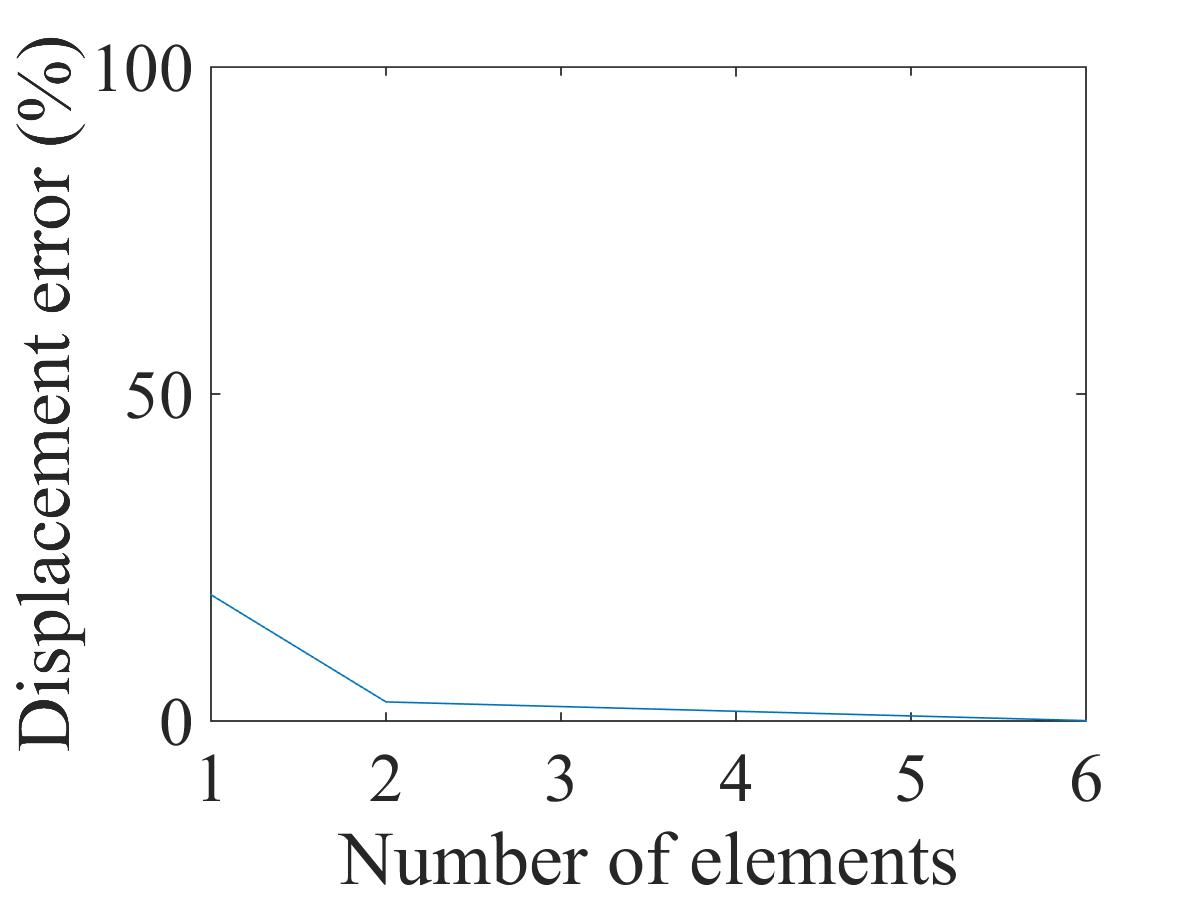
\includegraphics[width=6cm]{../Figure_files/27NodeBrick/error27brick_beam_different_element_number100.jpeg}
    \caption{Error scale 0\% - 100\%}
  \end{subfigure}
  \captionsetup{justification=centering,margin=2cm}
  \caption{27NodeBrick cantilever beam for different element number\\
    Displacement error   versus   Number of elements}
  \label{fig error 27NodeBrick cantilever beam for different element number}
\end{figure}


The ESSI model fei files for the table above are \href{https://github.com/yuan-energy/ESSI_Verification/blob/master/27NodeBrick/cantilever_different_element_number/cantilever_different_element_number.tar.gz?raw=true}{here}






\newpage
\subsection{Verification of 27NodeBrick circular plate with all edges simply supported}


Problem description: Diameter=20m, Height=1m, Force=100N, E=1E8Pa, $\nu=0.3$. 

The four edges are simply supported. 

The load is the uniform normal pressure on the whole plate. 


The plate flexural rigidity is 

\begin{equation}
  D=\frac{Eh^3}{12(1-\nu^2)}=\frac{10^8 N/m^2 \times 1^3 m^3 }{12 \times (1-0.3^2) }= 9.1575 \times 10^6 \ N\cdot m
\end{equation}

The theoretical solution\footnote{Stephen Timoshenko, Theory of plates and shells (2nd edition). MrGRAW-Hill Inc, page55, 1959.} is 

\begin{equation}
  d= \frac{(5+\nu)  q a^4}{64(1+\nu) D}=\frac{(5+0.3)\times 100 N/m^2 \times 10^4 m^4}{64\times(1+0.3) \times 9.1575 \times 10^6 \ N\cdot m}=6.956\times 10^{-3} m
\end{equation}



The 27NodeBrick were shown in Figure (\ref{fig 27NodeBrick edges simply supported circular plate with element side length 10m }) - (\ref{fig 27NodeBrick edges simply supported circular plate with element side length 0.25m }). 



\begin{figure}[H]
  \centering
  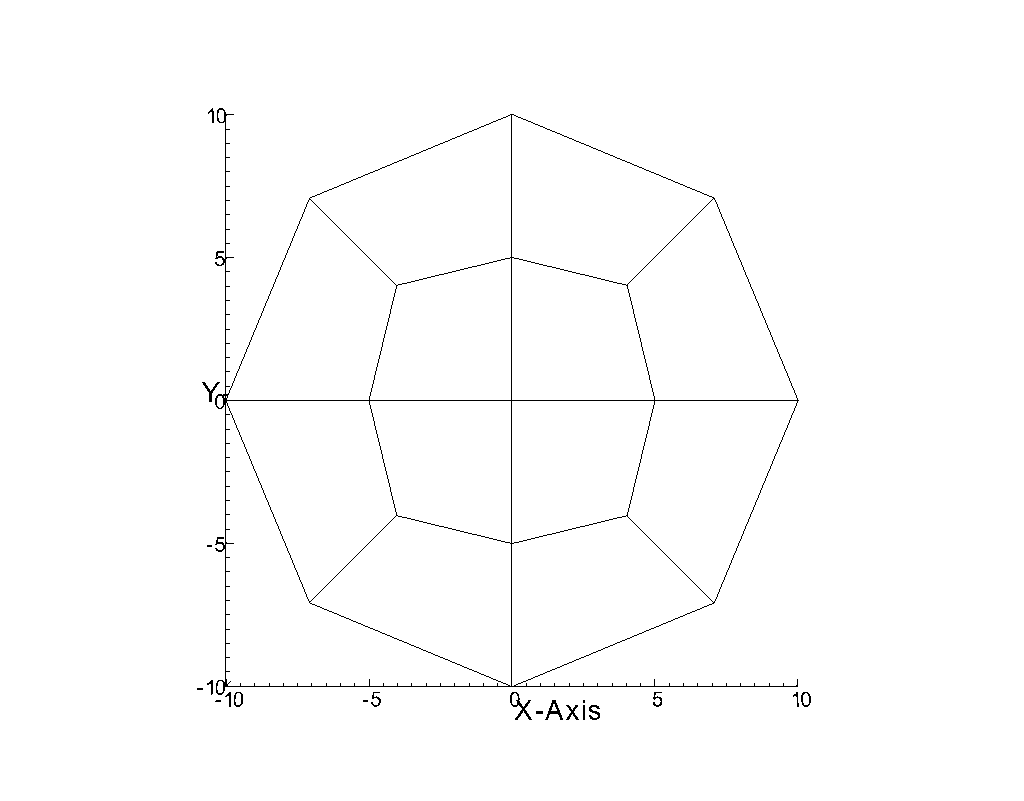
\includegraphics[width=11cm]{../Figure_files/27NodeBrick/circular_plate1.png}
  \caption{27NodeBrick edge simply supported circular plate with element side length 10m }
  \label{fig 27NodeBrick edges simply supported circular plate with element side length 10m }
\end{figure}

\newpage

\begin{figure}[H]
  \centering
  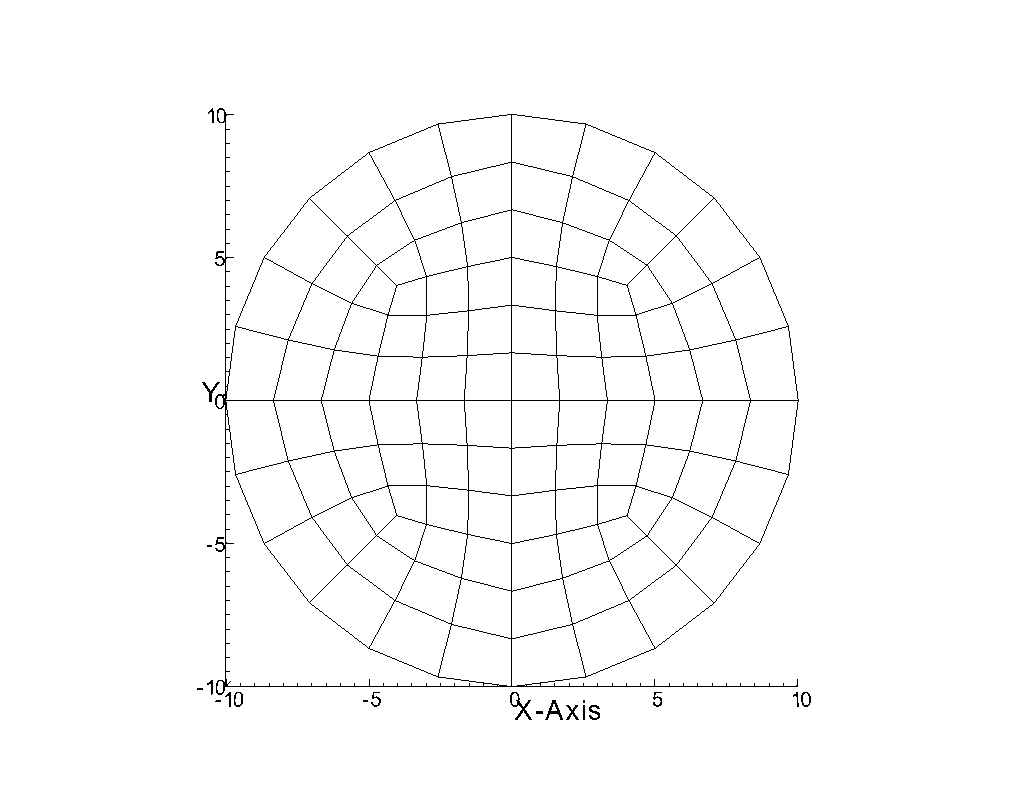
\includegraphics[width=11cm]{../Figure_files/27NodeBrick/circular_plate2.png}
  \caption{27NodeBrick edge simply supported circular plate with element side length 5m }
  \label{fig 27NodeBrick edges simply supported circular plate with element side length 5m }
\end{figure}


\begin{figure}[H]
  \centering
  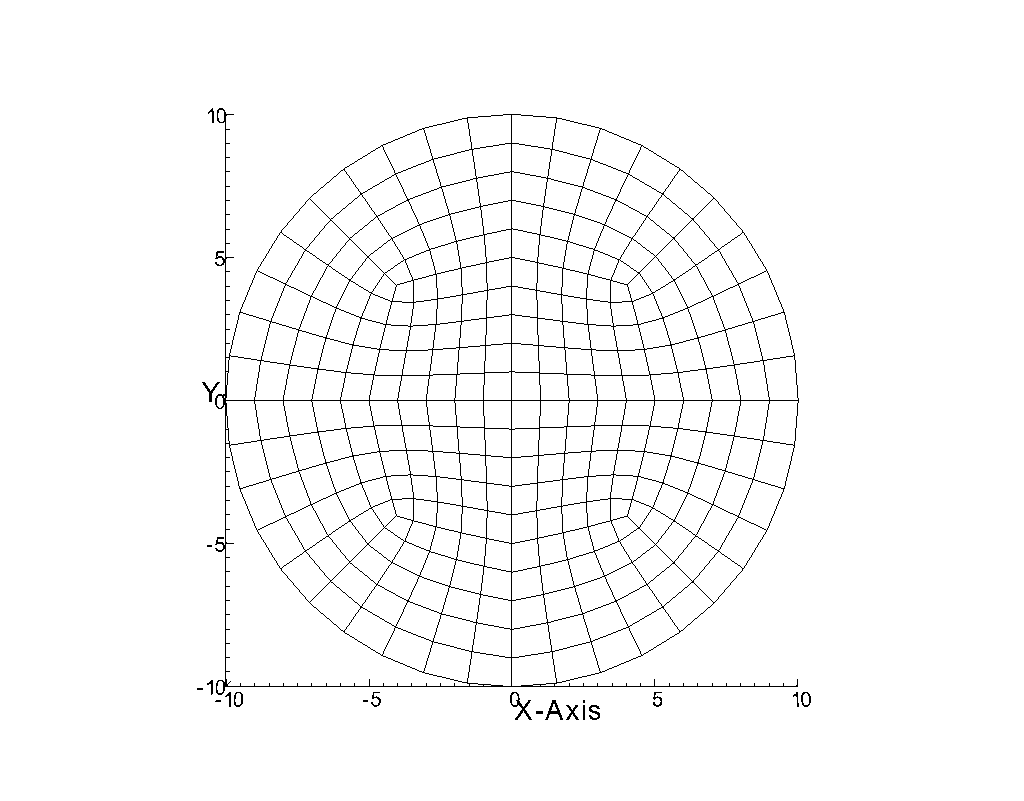
\includegraphics[width=11cm]{../Figure_files/27NodeBrick/circular_plate3.png}
  \caption{27NodeBrick edge simply supported circular plate with element side length 2m }
  \label{fig 27NodeBrick edges simply supported circular plate with element side length 2m }
\end{figure}

\newpage

\begin{figure}[H]
  \centering
  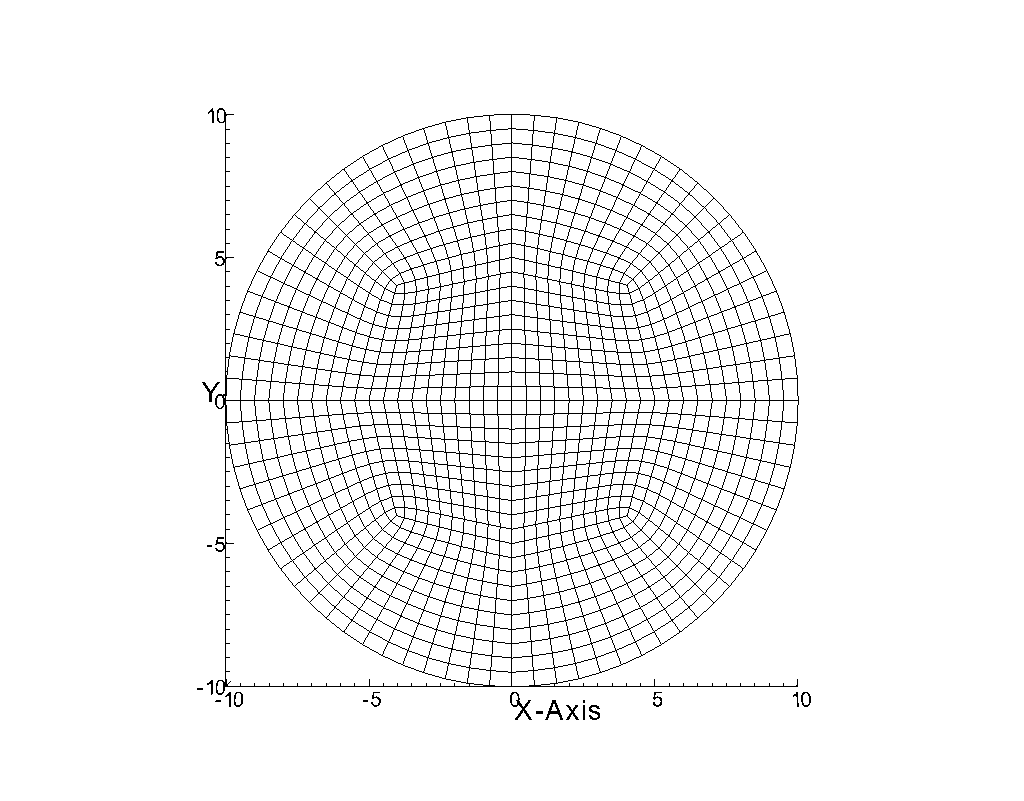
\includegraphics[width=11cm]{../Figure_files/27NodeBrick/circular_plate4.png}
  \caption{27NodeBrick edge simply supported circular plate with element side length 1m }
  \label{fig 27NodeBrick edges simply supported circular plate with element side length 1m }
\end{figure}


\begin{figure}[H]
  \centering
  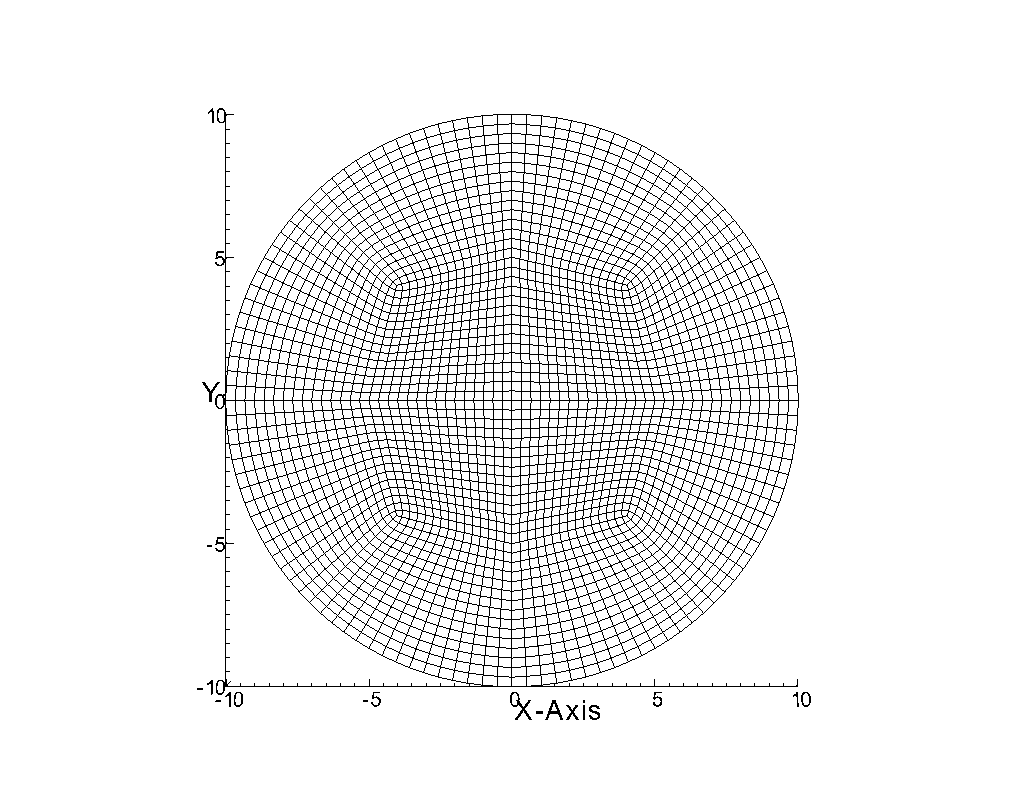
\includegraphics[width=11cm]{../Figure_files/27NodeBrick/circular_plate5.png}
  \caption{27NodeBrick edge simply supported circular plate with element side length 0.5m }
  \label{fig 27NodeBrick edges simply supported circular plate with element side length 0.5m }
\end{figure}

\newpage

\begin{figure}[H]
  \centering
  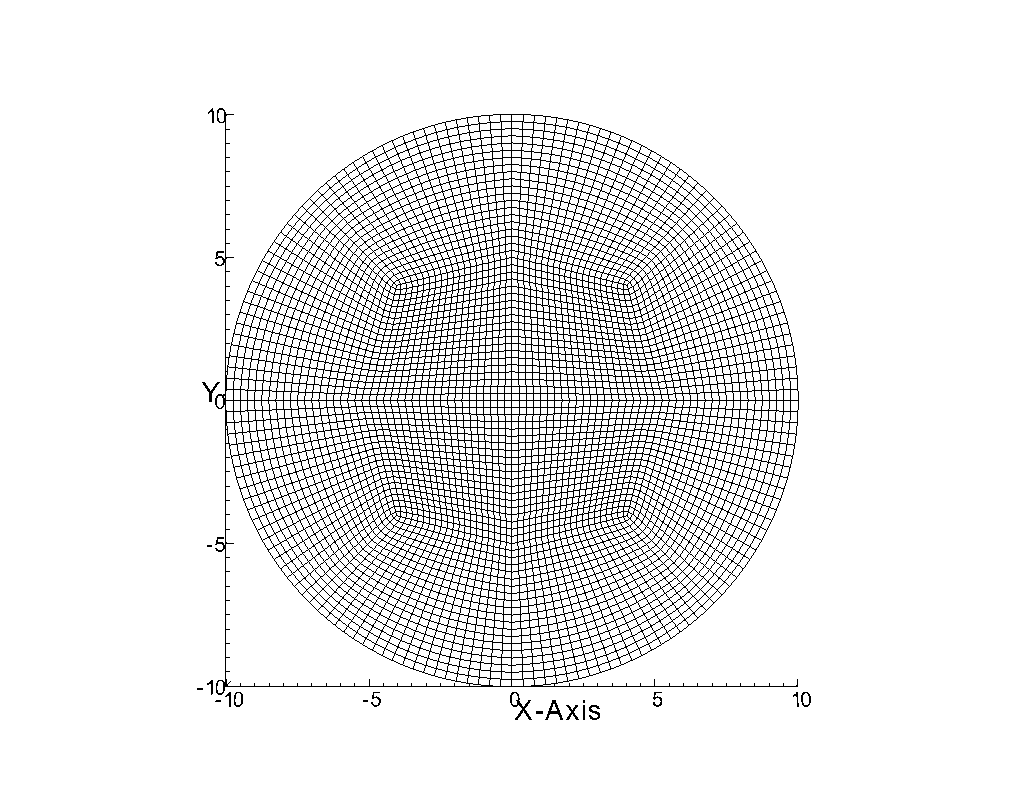
\includegraphics[width=11cm]{../Figure_files/27NodeBrick/circular_plate6.png}
  \caption{27NodeBrick edge simply supported circular plate with element side length 0.25m }
  \label{fig 27NodeBrick edges simply supported circular plate with element side length 0.25m }
\end{figure}





The results were listed in Table (\ref{table Results for 27NodeBrick cicular plate with four edges simply supported}).

\begin{table}[H]
  \centering
  \caption{Results for 27NodeBrick cicular plate with four edges simply supported}
  \label{table Results for 27NodeBrick cicular plate with four edges simply supported}
\begin{tabular}{|c|c|c|c|c|}
\hline
Element type        & 27NodeBrick     & 27NodeBrick     &  \multirow{3}{*}{\tabincell{c}{Theoretical \\ displacement}} \\ \cline{1-3}
Number of layers    & 2layers         & 4layers         &          \\ \cline{1-3}
Number of diameter divisions & Height:0.50$m$ & Height:0.25$m$ &          \\ \hline
4            & 7.259E-03 $m$ & 7.261E-03 $m$ & 6.956E-03 $m$ \\ \hline
12           & 7.083E-03 $m$ & 7.084E-03 $m$ & 6.956E-03 $m$ \\ \hline
20           & 7.064E-03 $m$ & 7.065E-03 $m$ & 6.956E-03 $m$ \\ \hline
40           & 7.018E-03 $m$ & 7.019E-03 $m$ & 6.956E-03 $m$ \\ \hline
60           & 7.029E-03 $m$ & 7.030E-03 $m$ & 6.956E-03 $m$ \\ \hline
80           & 7.032E-03 $m$ & 7.034E-03 $m$ & 6.956E-03 $m$ \\
\hline
\end{tabular}
\end{table}


The errors were listed in Table (\ref{table Errors for 27NodeBrick cicular plate with four edges simply supported}).

\begin{table}[H]
  \centering
  \caption{Errors for 27NodeBrick cicular plate with four edges simply supported}
  \label{table Errors for 27NodeBrick cicular plate with four edges simply supported}
  \begin{tabular}{|c|c|c|c|c|}
  \hline
  Element type     & 27NodeBrick     & 27NodeBrick      \\ \hline
  Number of layers      & 2layers         & 4layers          \\ \hline
  Number of diameter divisions & Height:0.50$m$ & Height:0.25$m$  \\ \hline
  4            & 4.36\% & 4.38\%      \\ \hline
  12           & 1.82\% & 1.83\%      \\ \hline
  20           & 1.56\% & 1.57\%      \\ \hline
  40           & 0.88\% & 0.90\%      \\ \hline
  60           & 1.04\% & 1.06\%      \\ \hline
  80           & 1.09\% & 1.11\%      \\
  \hline
  \end{tabular}
\end{table}

% \begin{figure}[H]
%   \centering
%   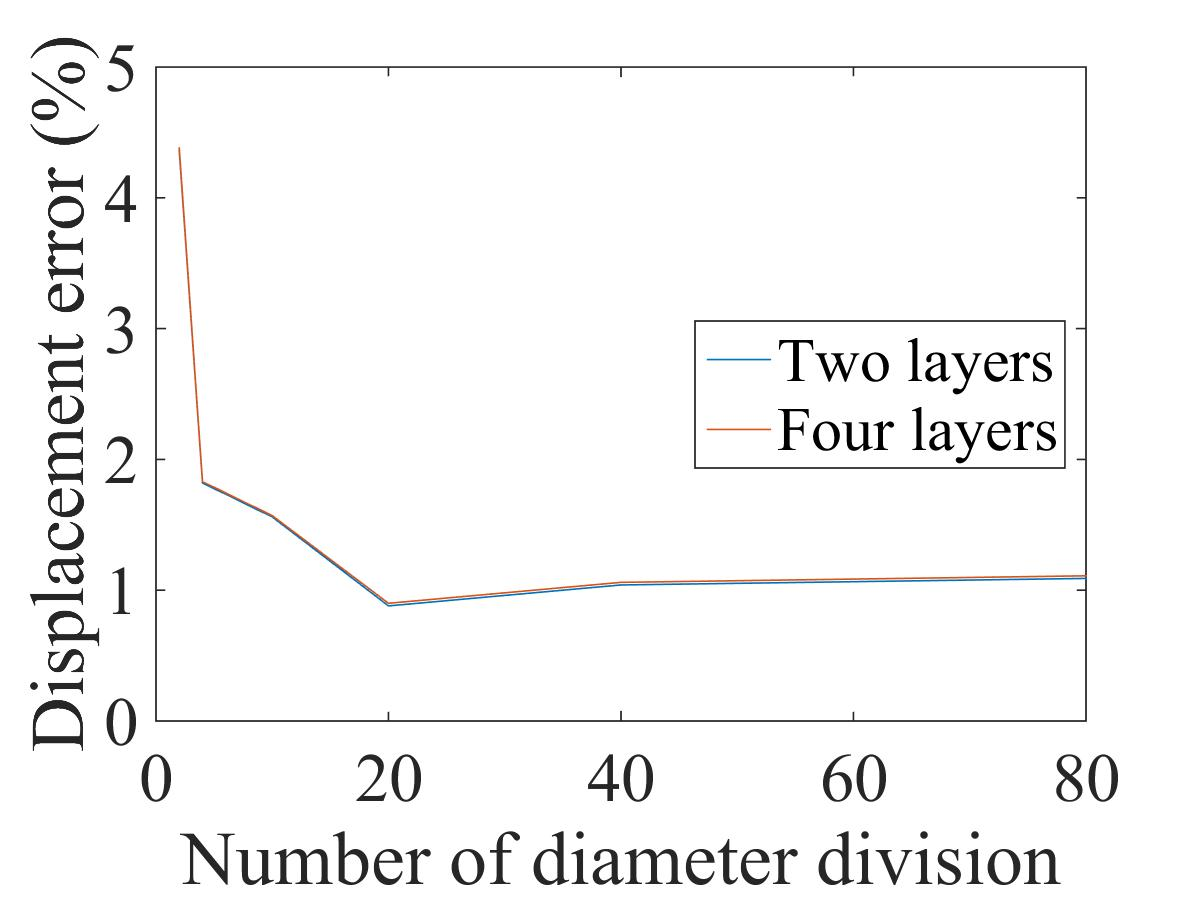
\includegraphics[width=9cm]{../Figure_files/27NodeBrick/error27brick_circular_plate_simply_supported.jpeg}
%   % \caption{}
%   % \label{}
% \end{figure}

The errors were plotted in Figure (\ref{fig 27NodeBrick circular plate with four edge simply supported}).
\begin{figure}[H]
  % \centering
  \begin{subfigure}{0.5\textwidth}
    \centering
    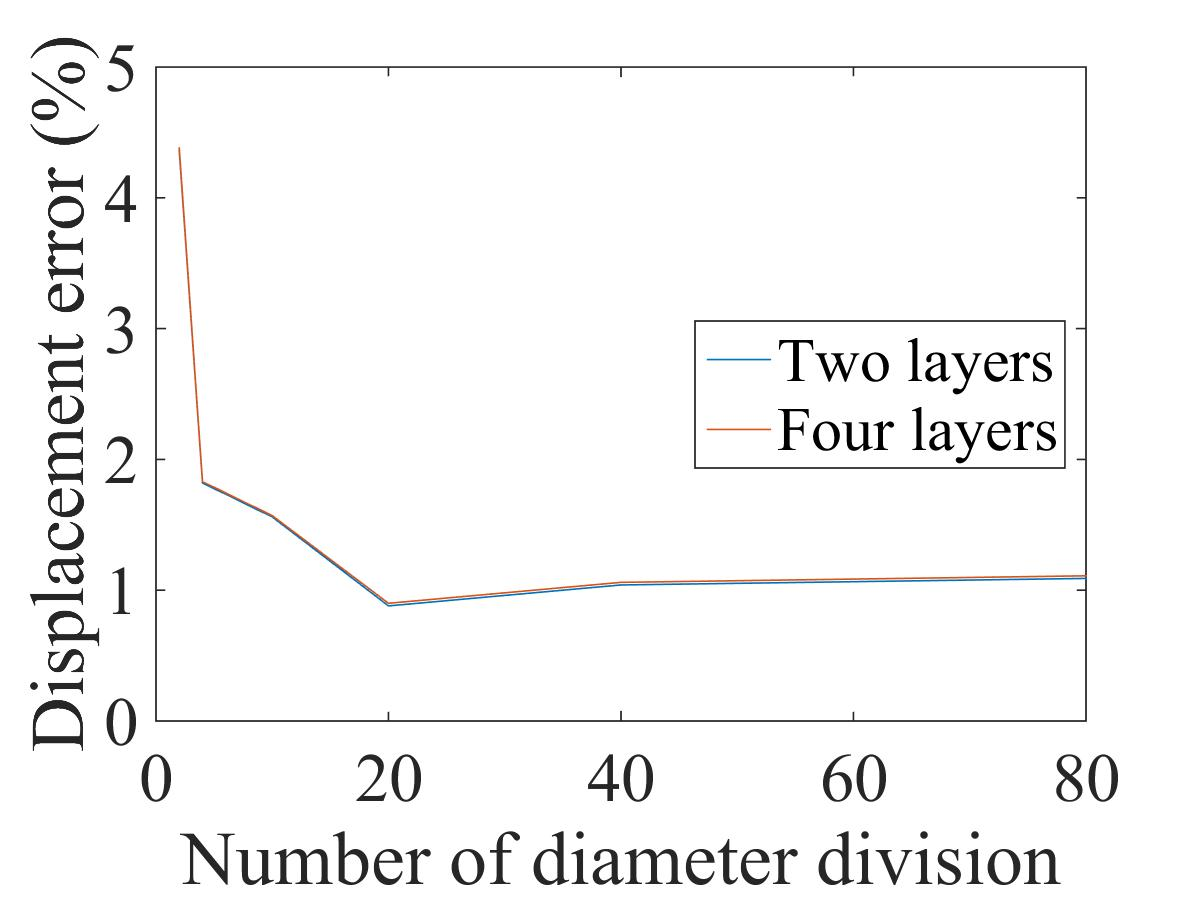
\includegraphics[width=6cm]{../Figure_files/27NodeBrick/error27brick_circular_plate_simply_supported.jpeg}
    \caption{Error scale 0\% - 5\%}
  \end{subfigure}
  \begin{subfigure}{0.5\textwidth}
    \centering
    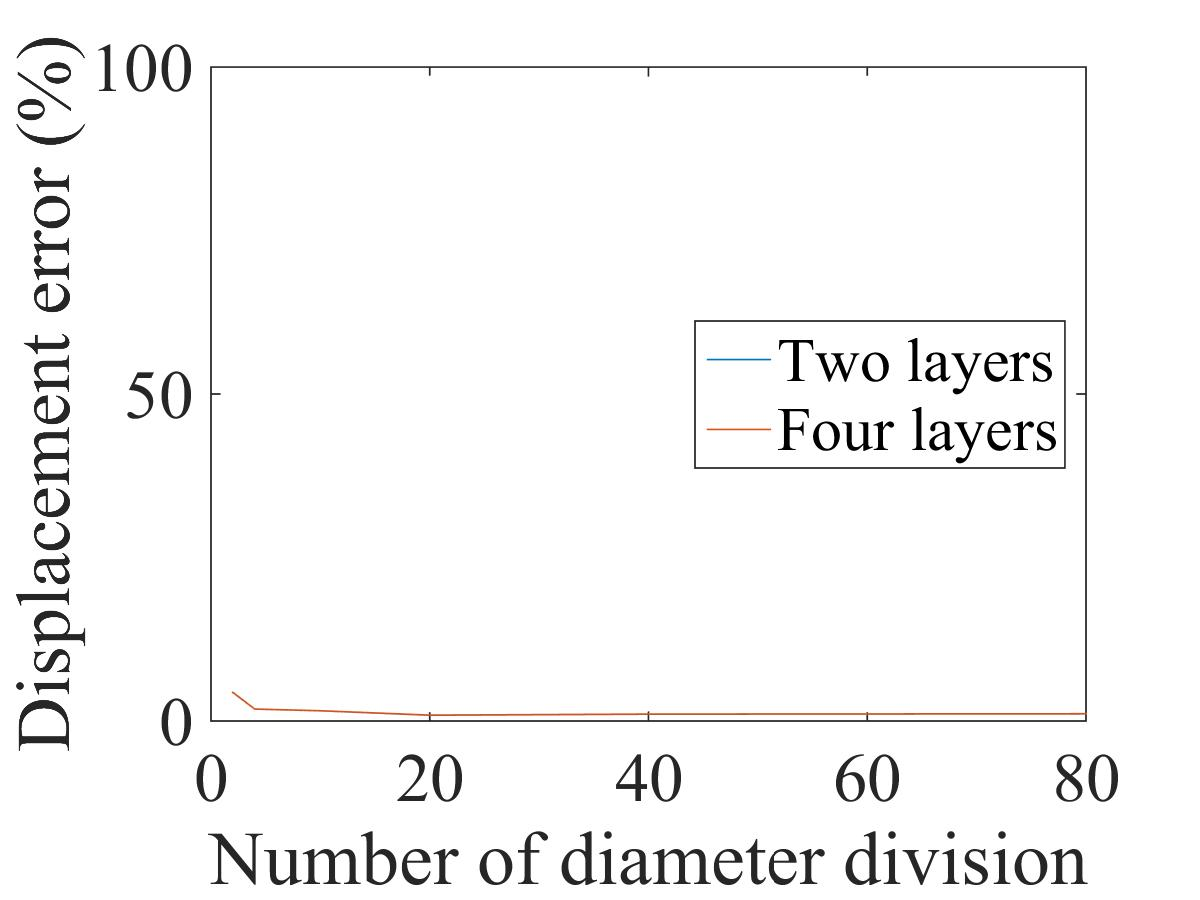
\includegraphics[width=6cm]{../Figure_files/27NodeBrick/error27brick_circular_plate_simply_supported100.jpeg}
    \caption{Error scale 0\% - 100\%}
  \end{subfigure}
  \captionsetup{justification=centering,margin=3cm}
  \caption{27NodeBrick circular plate with edge simply supported\\
      Displacement error   versus   Number of side division}
  \label{fig 27NodeBrick circular plate with four edge simply supported}
\end{figure}






The ESSI model fei files for the table above are \href{https://github.com/yuan-energy/ESSI_Verification/blob/master/27NodeBrick/circular_plate_simply_support/circular_plate_simply_support.tar.gz?raw=true}{here}







% 27NodeBrick ends
% 27NodeBrick ends
% 27NodeBrick ends
% 27NodeBrick ends
% 27NodeBrick ends
% 27NodeBrick ends
% 27NodeBrick ends
% 27NodeBrick ends

% 4NodeANDES starts
% 4NodeANDES starts
% 4NodeANDES starts
% 4NodeANDES starts
% 4NodeANDES starts
% 4NodeANDES starts


















\newpage
\begin{center}
  \Large\textbf{Verification for 4NodeANDES}
\end{center}


\vskip 24pt

\section{Verification of 4NodeANDES elements}
\subsection{Verification of 4NodeANDES cantilever beams}





Problem description: Length=6m, Width=1m, Height=1m, Force=100N, E=1E8Pa, $\nu=0.0$. The force direction was shown in Figure (\ref{fig Problem description for cantilever 4}). 

\begin{figure}[H]
  \centering
  \includegraphics[width=7cm]{../Figure_files/4NodeANDES/cantilever_6.pdf}
  \caption{Problem description for cantilever beams}
  \label{fig Problem description for cantilever 4}
\end{figure}


Theoretical displacement (bending and shear deformation):
\begin{equation}
  \begin{aligned}
  d &=\frac{FL^3}{3EI}+\frac{FL}{GA} \\ 
    &= \frac{100 N \times 6^3 m^3}{3\times 10^8 N/m^2 \times \frac{1}{12} m^4}+ 
    \frac{100 N\times 6 m}{5\times 10^7 N/m^2\times 1 m^2} \\ 
    &=8.64\times 10^{-4} m + 0.12 \times 10^{-4} m  \\
   & =8.76\times 10^{-4} \ m
   \end{aligned}
\end{equation}



4NodeANDES element model:

\vskip 12pt

\begin{itemize}
  \item \textbf{\emph{Force direction: perpendicular to plane (bending)}}
\end{itemize}
When the force direction is perpendicular to the plane, only the bending deformation is calculated in 4NodeANDES elements. 


The 4NodeANDES elements were shown in Figure (\ref{fig 4NodeANDES elements for cantilever beams under force perpendicular to plane}).

\begin{figure}[H]
  \centering
  \begin{subfigure}{0.5\textwidth}
    \centering
    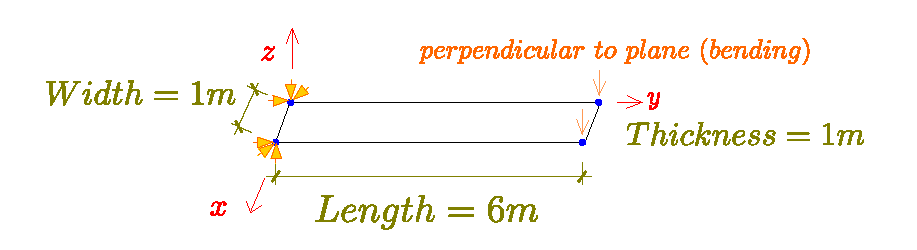
\includegraphics[width=9cm]{../Figure_files/4NodeANDES/beam_ANDES_xy_bending_1div.pdf}
    \caption{One 4NodeANDES element}
  \end{subfigure}
  \vskip 8pt
  \begin{subfigure}{0.5\textwidth}
    \centering
    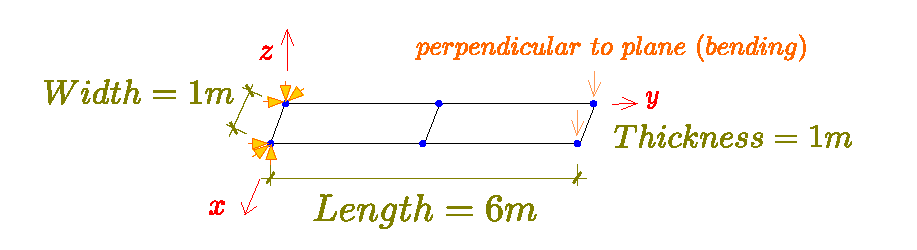
\includegraphics[width=9cm]{../Figure_files/4NodeANDES/beam_ANDES_xy_bending_2div.pdf}
    \caption{Two 4NodeANDES elements}
  \end{subfigure}
  \vskip 8pt
  \begin{subfigure}{0.5\textwidth}
    \centering
    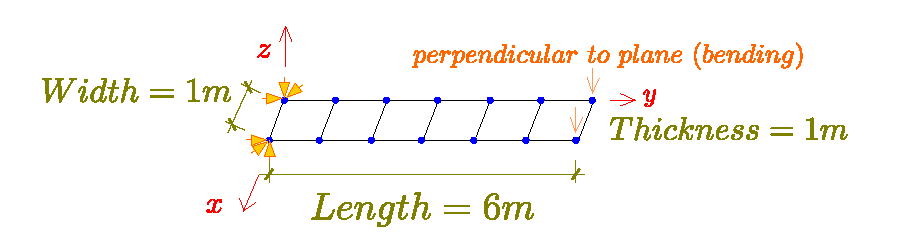
\includegraphics[width=9cm]{../Figure_files/4NodeANDES/beam_ANDES_xy_bending_6div.pdf}
    \caption{Six 4NodeANDES elements}
  \end{subfigure}
  \captionsetup{justification=centering,margin=3cm}
  \caption{4NodeANDES elements for cantilever beams under force perpendicular to plane}
  \label{fig 4NodeANDES elements for cantilever beams under force perpendicular to plane}
\end{figure}


% One element:

% \begin{figure}[H]
%   \centering
%   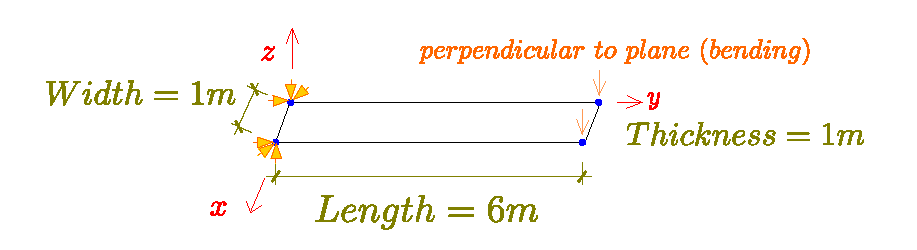
\includegraphics[width=9cm]{../Figure_files/4NodeANDES/beam_ANDES_xy_bending_1div.pdf}
%   % \caption{}
%   % \label{}
% \end{figure}

% Two elements: 

% \begin{figure}[H]
%   \centering
%   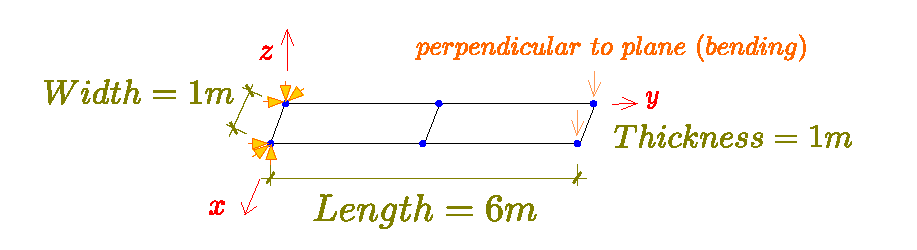
\includegraphics[width=9cm]{../Figure_files/4NodeANDES/beam_ANDES_xy_bending_2div.pdf}
%   % \caption{}
%   % \label{}
% \end{figure}


% Six elements: 

% \begin{figure}[H]
%   \centering
%   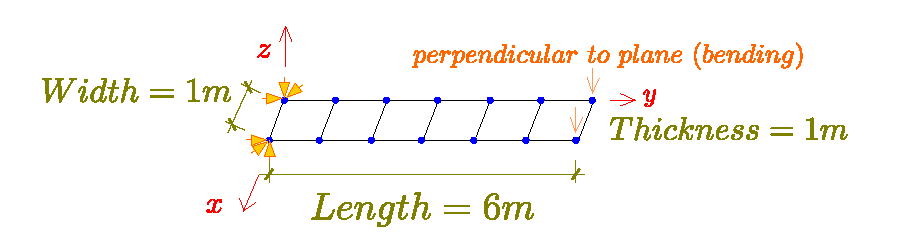
\includegraphics[width=9cm]{../Figure_files/4NodeANDES/beam_ANDES_xy_bending_6div.pdf}
%   % \caption{}
%   % \label{}
% \end{figure}

\begin{itemize}
  \item \textbf{\emph{Force direction: inplane force }}
\end{itemize}
When the force direction is inplane, both the bending and shear deformation are calculated in 4NodeANDES elements. 


The 4NodeANDES elements under inplane force were shown in Figure (\ref{fig 4NodeANDES elements for cantilever beams under inplane force}).

\begin{figure}[H]
  \centering
  \begin{subfigure}{0.5\textwidth}
    \centering
    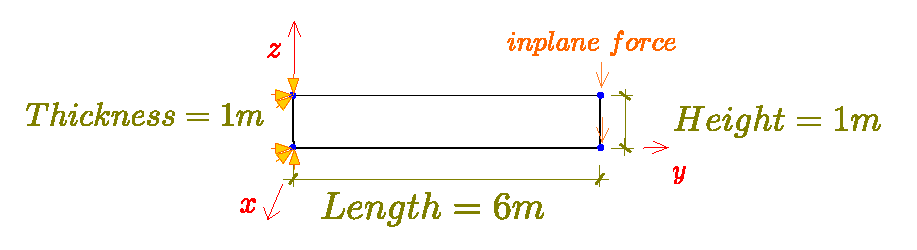
\includegraphics[width=9cm]{../Figure_files/4NodeANDES/beam_ANDES_yz_inPlane_1div.pdf}
    \caption{One 4NodeANDES element}
  \end{subfigure}
  \vskip 8pt
  \begin{subfigure}{0.5\textwidth}
    \centering
    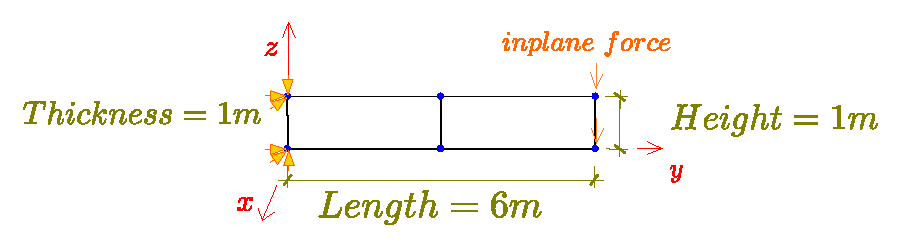
\includegraphics[width=9cm]{../Figure_files/4NodeANDES/beam_ANDES_yz_inPlane_2div.pdf}
    \caption{Two 4NodeANDES elements}
  \end{subfigure}
  \vskip 8pt
  \begin{subfigure}{0.5\textwidth}
    \centering
    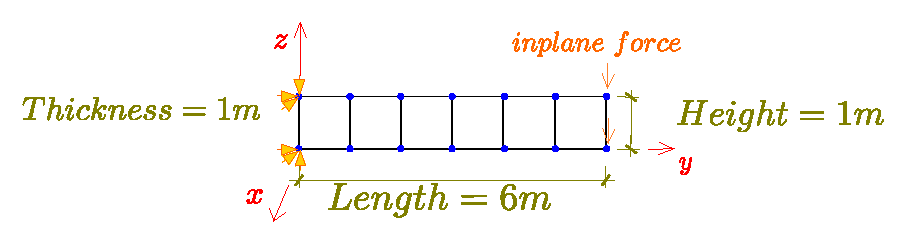
\includegraphics[width=9cm]{../Figure_files/4NodeANDES/beam_ANDES_yz_inPlane_6div.pdf}
    \caption{Six 4NodeANDES elements}
  \end{subfigure}
  \captionsetup{justification=centering,margin=3cm}
  \caption{4NodeANDES elements for cantilever beams under inplane force}
  \label{fig 4NodeANDES elements for cantilever beams under inplane force}
\end{figure}


% One element:

% \begin{figure}[H]
%   \centering
%   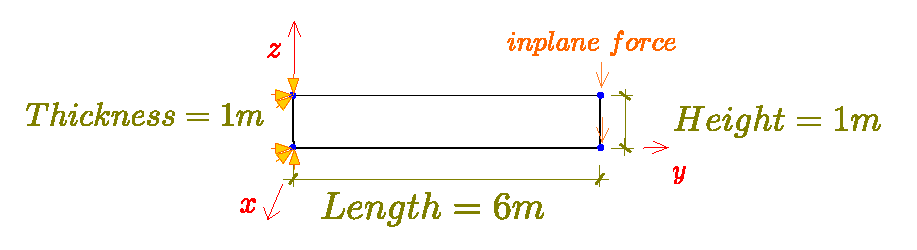
\includegraphics[width=9cm]{../Figure_files/4NodeANDES/beam_ANDES_yz_inPlane_1div.pdf}
%   % \caption{}
%   % \label{}
% \end{figure}

% Two elements: 
% \begin{figure}[H]
%   \centering
%   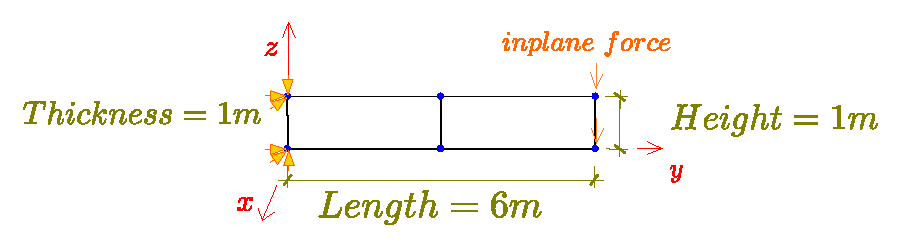
\includegraphics[width=9cm]{../Figure_files/4NodeANDES/beam_ANDES_yz_inPlane_2div.pdf}
%   % \caption{}
%   % \label{}
% \end{figure}

% Six elements: 

% \begin{figure}[H]
%   \centering
%   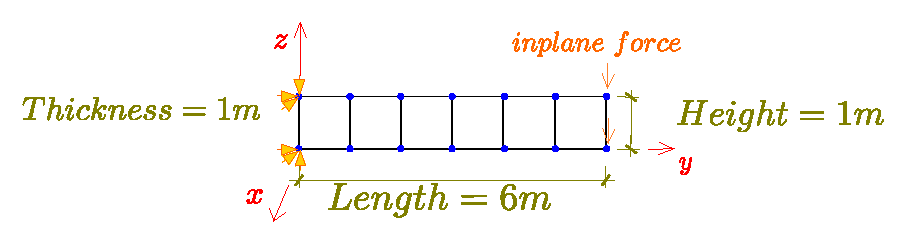
\includegraphics[width=9cm]{../Figure_files/4NodeANDES/beam_ANDES_yz_inPlane_6div.pdf}
%   % \caption{}
%   % \label{}
% \end{figure}



The ESSI results for the force \textbf{\emph{perpendicular to plane (bending)}} were listed in Table (\ref{table 4NodeANDES cantilever beams results for different element number}). 
The theoretical solution is 8.760E-04 $m$.
\begin{table}[H]
  \centering
    \captionsetup{justification=centering,margin=2cm}
      \caption{Results for 4NodeANDES cantilever beams under the force perpendicular to plane (bending)}
    \label{table 4NodeANDES cantilever beams results for different element number}
    \begin{tabular}{|c|c|c|c|}
      \hline
      Element number & 1        & 2        & 6         \\  \hline
      4NodeANDES     & 6.56E-04 $m$ & 8.27E-04 $m$ & 8.86E-04 $m$     \\ \hline
      Error          & 25.14\%  & 5.62\%   & 1.11\%     \\ 
      \hline 
    \end{tabular}
\end{table}
The ESSI results for the \textbf{\emph{inplane force}} were listed in Table (\ref{table 4NodeANDES cantilever beams results for different element number 2}). 

The theoretical solution is 8.760E-04 $m$.


\begin{table}[H]
  \centering
      \captionsetup{justification=centering,margin=2cm}
      \caption{Results for 4NodeANDES cantilever beams under the inplane force}
    \label{table 4NodeANDES cantilever beams results for different element number 2}
    \begin{tabular}{|c|c|c|c|}
      \hline
      Element number & 1        & 2        & 6         \\  \hline
      4NodeANDES     &6.70E-04 $m$& 8.27E-04 $m$& 8.64E-04 $m$     \\ \hline
      Error          &  23.56\%  & 5.63\%   & 1.38\%          \\ 
      \hline 
    \end{tabular}
\end{table}

% \begin{figure}[H]
%   \centering
%   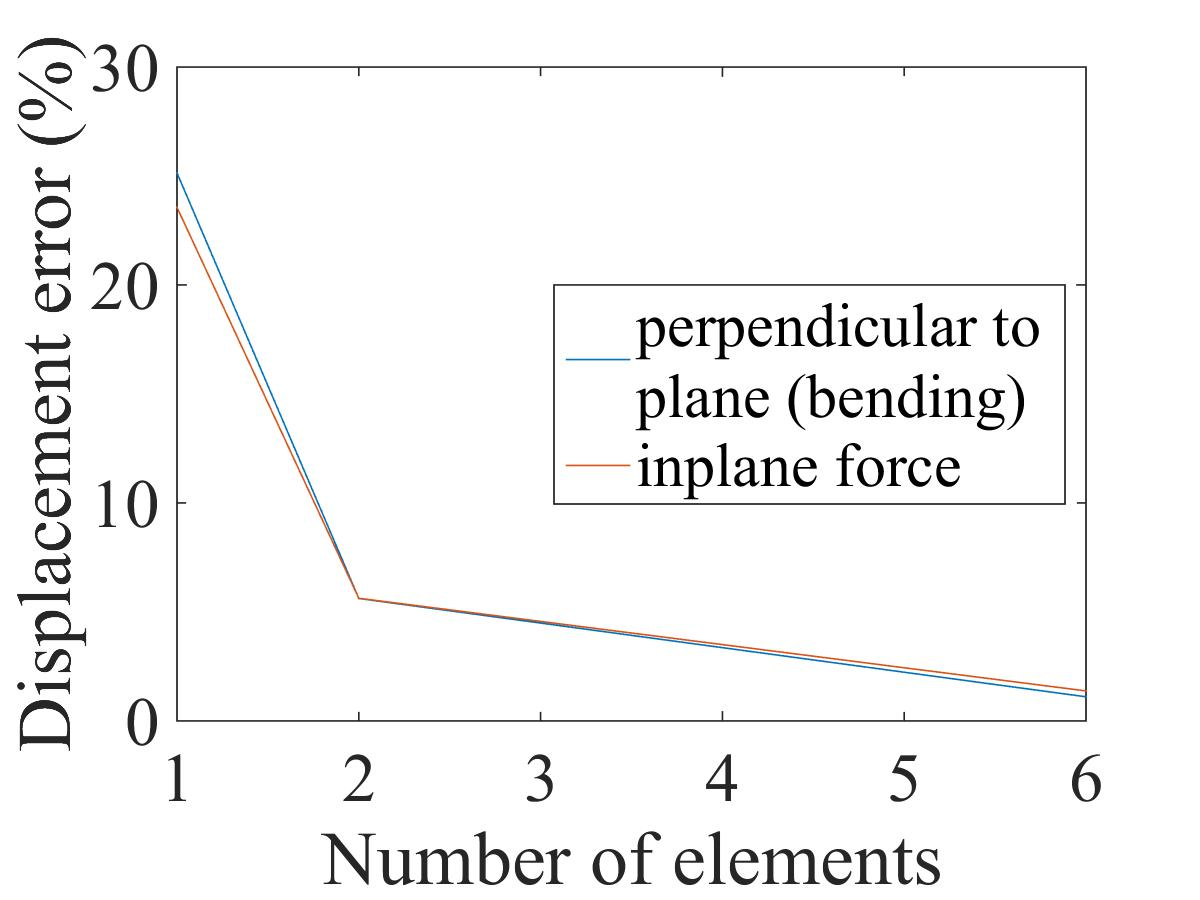
\includegraphics[width=9cm]{../Figure_files/4NodeANDES/error4andes_beam_different_element_number.jpeg}
%   % \caption{}
%   % \label{}
% \end{figure}

The errors were plotted in Figure (\ref{fig error 4NodeANDES cantilever beam for different element number}).

\begin{figure}[H]
  % \centering
  \begin{subfigure}{0.5\textwidth}
    \centering
    \includegraphics[width=6cm]{../Figure_files/4NodeANDES/error4andes_beam_different_element_number.jpeg}
    \caption{Error scale 0\% - 30\%}
  \end{subfigure}
  \begin{subfigure}{0.5\textwidth}
    \centering
    \includegraphics[width=6cm]{../Figure_files/4NodeANDES/error4andes_beam_different_element_number100.jpeg}
    \caption{Error scale 0\% - 100\%}
  \end{subfigure}
  \captionsetup{justification=centering,margin=2cm}
  \caption{4NodeANDES cantilever beam for different element number\\
    Displacement error   versus   Number of elements}
  \label{fig error 4NodeANDES cantilever beam for different element number}
\end{figure}


The ESSI model fei files for the table above are \href{https://github.com/yuan-energy/ESSI_Verification/blob/master/4NodeANDES/cantilever_different_element_number/cantilever_different_element_number.tar.gz?raw=true}{here}
















\newpage
\subsection{Verification of 4NodeANDES circular plate with all edges simply supported}


Problem description: Diameter=20m, Height=1m, Force=100N, E=1E8Pa, $\nu=0.3$. 

The four edges are simply supported. 

The load is the uniform normal pressure on the whole plate. 


The plate flexural rigidity is 

\begin{equation}
  D=\frac{Eh^3}{12(1-\nu^2)}=\frac{10^8 N/m^2 \times 1^3 m^3 }{12 \times (1-0.3^2) }= 9.1575 \times 10^6 \ N\cdot m
\end{equation}

The theoretical solution\footnote{Stephen Timoshenko, Theory of plates and shells (2nd edition). MrGRAW-Hill Inc, page55, 1959.} is 

\begin{equation}
  d= \frac{(5+\nu)  q a^4}{64(1+\nu) D}=\frac{(5+0.3)\times 100 N/m^2 \times 10^4 m^4}{64\times(1+0.3) \times 9.1575 \times 10^6 \ N\cdot m}=6.956\times 10^{-3} m
\end{equation}


The 4NodeANDES were shown in Figure (\ref{fig 4NodeANDES edges simply supported circular plate with element side length 10m }) - (\ref{fig 4NodeANDES edges simply supported circular plate with element side length 0.25m }). 



\begin{figure}[H]
  \centering
  \includegraphics[width=11cm]{../Figure_files/4NodeANDES/circular_plate1.png}
  \caption{4NodeANDES edge simply supported circular plate with element side length 10m }
  \label{fig 4NodeANDES edges simply supported circular plate with element side length 10m }
\end{figure}

\newpage

\begin{figure}[H]
  \centering
  \includegraphics[width=11cm]{../Figure_files/4NodeANDES/circular_plate2.png}
  \caption{4NodeANDES edge simply supported circular plate with element side length 5m }
  \label{fig 4NodeANDES edges simply supported circular plate with element side length 5m }
\end{figure}


\begin{figure}[H]
  \centering
  \includegraphics[width=11cm]{../Figure_files/4NodeANDES/circular_plate3.png}
  \caption{4NodeANDES edge simply supported circular plate with element side length 2m }
  \label{fig 4NodeANDES edges simply supported circular plate with element side length 2m }
\end{figure}

\newpage

\begin{figure}[H]
  \centering
  \includegraphics[width=11cm]{../Figure_files/4NodeANDES/circular_plate4.png}
  \caption{4NodeANDES edge simply supported circular plate with element side length 1m }
  \label{fig 4NodeANDES edges simply supported circular plate with element side length 1m }
\end{figure}


\begin{figure}[H]
  \centering
  \includegraphics[width=11cm]{../Figure_files/4NodeANDES/circular_plate5.png}
  \caption{4NodeANDES edge simply supported circular plate with element side length 0.5m }
  \label{fig 4NodeANDES edges simply supported circular plate with element side length 0.5m }
\end{figure}

\newpage

\begin{figure}[H]
  \centering
  \includegraphics[width=11cm]{../Figure_files/4NodeANDES/circular_plate6.png}
  \caption{4NodeANDES edge simply supported circular plate with element side length 0.25m }
  \label{fig 4NodeANDES edges simply supported circular plate with element side length 0.25m }
\end{figure}





The results were listed in Table (\ref{table Results for 4NodeANDES cicular plate with four edges simply supported}).

\begin{table}[H]
  \centering
  \caption{Results for 4NodeANDES cicular plate with four edges simply supported}
  \label{table Results for 4NodeANDES cicular plate with four edges simply supported}
\begin{tabular}{|c|c|c|}
\hline
Element type     & 4NodeANDES        &  \multirow{2}{*}{\tabincell{c}{Theoretical \\ displacement}} \\ \cline{1-2}
Element side length & Height:1.00$m$ &        \\ \hline
10$m$            & 7.50E-003 $m$ & 6.956E-03 $m$ \\ \hline
5$m$             & 7.29E-003 $m$ & 6.956E-03 $m$ \\ \hline
2$m$             & 7.25E-003 $m$ & 6.956E-03 $m$ \\ \hline
1$m$             & 7.23E-003 $m$ & 6.956E-03 $m$ \\ \hline
0.5$m$           & 7.22E-003 $m$ & 6.956E-03 $m$ \\ \hline
0.25$m$          & 7.22E-003 $m$ & 6.956E-03 $m$ \\
\hline
\end{tabular}
\end{table}


The errors were listed in Table (\ref{table Errors for 4NodeANDES cicular plate with four edges simply supported}).

\begin{table}[H]
  \centering
  \caption{Errors for 4NodeANDES cicular plate with four edges simply supported}
  \label{table Errors for 4NodeANDES cicular plate with four edges simply supported}
\begin{tabular}{|c|c|}
\hline
Element type     & 4NodeANDES          \\ \hline
Element side length & Height:1.00$m$   \\ \hline
10$m$            & 7.75\%        \\ \hline
5$m$             & 4.73\%        \\ \hline
2$m$             & 4.15\%        \\ \hline
1$m$             & 3.89\%        \\ \hline
0.5$m$           & 3.84\%        \\ \hline
0.25$m$          & 3.82\%       \\
\hline
\end{tabular}
\end{table}

% \begin{figure}[H]
%   \centering
%   \includegraphics[width=9cm]{../Figure_files/4NodeANDES/error4andes_circular_plate_simply_supported.jpeg}
%   % \caption{}
%   % \label{}
% \end{figure}
The errors were plotted in Figure (\ref{fig 4NodeANDES circular plate with four edge simply supported}).
\begin{figure}[H]
  % \centering
  \begin{subfigure}{0.5\textwidth}
    \centering
    \includegraphics[width=6cm]{../Figure_files/4NodeANDES/error4andes_circular_plate_simply_supported.jpeg}
    \caption{Error scale 0\% - 8\%}
  \end{subfigure}
  \begin{subfigure}{0.5\textwidth}
    \centering
    \includegraphics[width=6cm]{../Figure_files/4NodeANDES/error4andes_circular_plate_simply_supported100.jpeg}
    \caption{Error scale 0\% - 100\%}
  \end{subfigure}
  \captionsetup{justification=centering,margin=3cm}
  \caption{4NodeANDES circular plate with edge simply supported\\
      Displacement error   versus   Number of side division}
  \label{fig 4NodeANDES circular plate with four edge simply supported}
\end{figure}


The ESSI model fei files for the table above are \href{https://github.com/yuan-energy/ESSI_Verification/blob/master/4NodeANDES/circular_plate_simply_support/circular_plate_simply_support.tar.gz?raw=true}{here}















%-------------------------------------------------------------------------------------------------------------%
%-------------------------------------------------------------------------------------------------------------%

\end{document}


        10        20        30        40        50        60        70        80
12345678901234567890123456789012345678901234567890123456789012345678901234567890
